\hypertarget{Classes_8c}{
\section{Classes.c File Reference}
\label{Classes_8c}\index{Classes.c@{Classes.c}}
}
{\tt \#include \char`\"{}party.h\char`\"{}}\par


Include dependency graph for Classes.c:\begin{figure}[H]
\begin{center}
\leavevmode
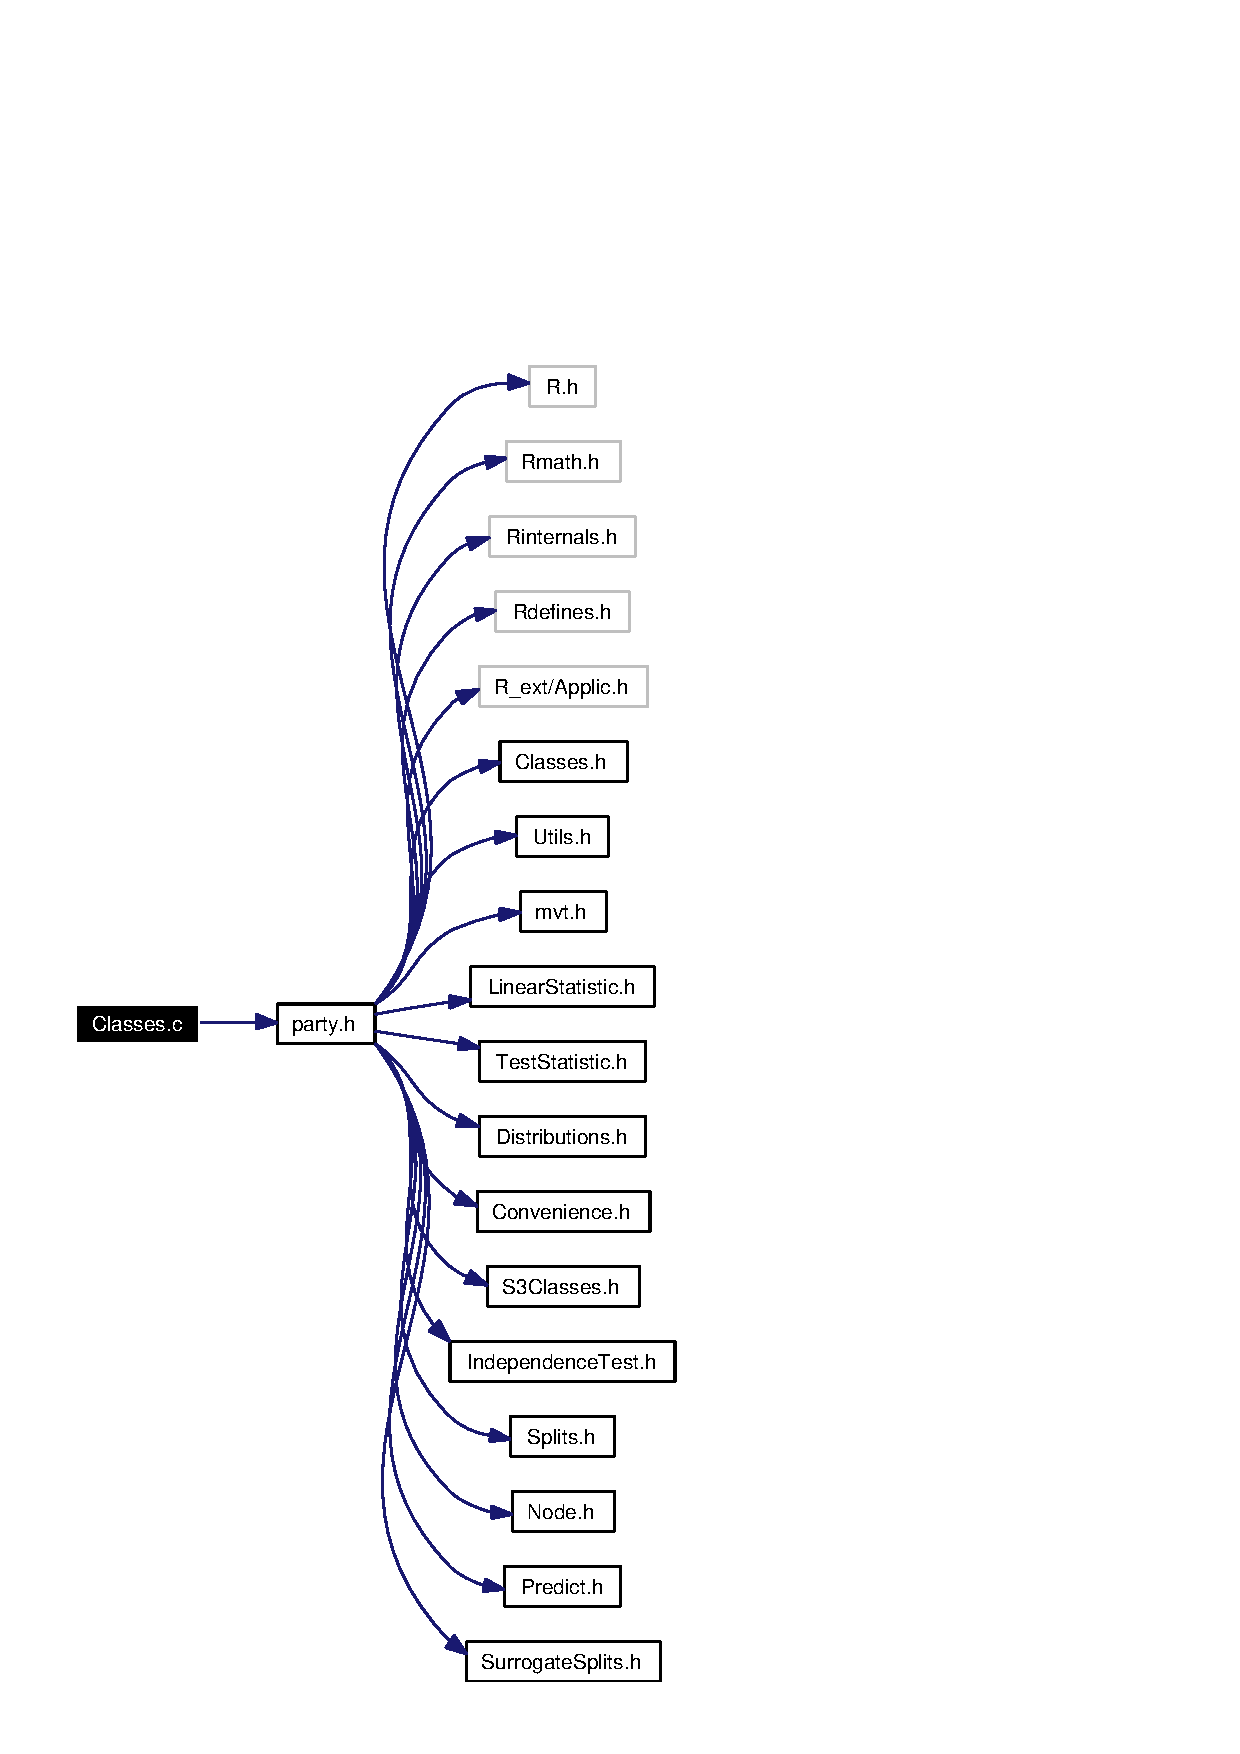
\includegraphics[width=162pt]{Classes_8c__incl}
\end{center}
\end{figure}
\subsection*{Functions}
\begin{CompactItemize}
\item 
SEXP \hyperlink{Classes_8c_ddd65d92d4da9d50911d5f33130e7887}{party\_\-init} (void)
\item 
int \hyperlink{Classes_8c_8bc9164a2291bb7f61c12b79f6bc7c5f}{get\_\-dimension} (SEXP object)
\item 
int \hyperlink{Classes_8c_847e08eb9fce554539de3106ea03e9e2}{get\_\-teststat} (SEXP object)
\item 
int \hyperlink{Classes_8c_309a9064403a71aba540cad646ba5854}{get\_\-pvalue} (SEXP object)
\item 
double \hyperlink{Classes_8c_aa5df349ffd6e5faccab211ac972722b}{get\_\-tol} (SEXP object)
\item 
int \hyperlink{Classes_8c_b0fc0f7fb33f87cfa58cb8c617d946a1}{get\_\-maxpts} (SEXP object)
\item 
double \hyperlink{Classes_8c_4e2233c1c47758c555f99235f60984f0}{get\_\-abseps} (SEXP object)
\item 
double \hyperlink{Classes_8c_a17053ff24db1859af60e2d71baf924c}{get\_\-releps} (SEXP object)
\item 
double \hyperlink{Classes_8c_024b7f74a61afa9b3eb465a98f35584c}{get\_\-minsplit} (SEXP object)
\item 
double \hyperlink{Classes_8c_f7aaeccefe1bfbb1737ac3403a85c8e9}{get\_\-minprob} (SEXP object)
\item 
double \hyperlink{Classes_8c_0794d3cb26a60105140165d6dea3d70d}{get\_\-minbucket} (SEXP object)
\item 
SEXP \hyperlink{Classes_8c_20a55355301b5f90ec48b9114d1ff597}{get\_\-transformation} (SEXP object, int variable)
\item 
SEXP \hyperlink{Classes_8c_9ec50a13a7c7e82143cced16ff4f3968}{get\_\-test\_\-trafo} (SEXP object)
\item 
SEXP \hyperlink{Classes_8c_b86d70ff194260cc9bd391d3ff55b157}{get\_\-predict\_\-trafo} (SEXP object)
\item 
SEXP \hyperlink{Classes_8c_0f91efa916e815ec7d90c6f9516f18e4}{get\_\-variable} (SEXP object, int variable)
\item 
int \hyperlink{Classes_8c_f836613ade2cdc01c401b574fc1e7fdb}{is\_\-nominal} (SEXP object, int variable)
\item 
int \hyperlink{Classes_8c_53608524b90af1655d49496ec5ccbd47}{is\_\-ordinal} (SEXP object, int variable)
\item 
int \hyperlink{Classes_8c_2ea962f10f7adde8ad25429e15cad9d3}{is\_\-censored} (SEXP object, int variable)
\item 
int \hyperlink{Classes_8c_50548fbe6024d9a7118db3fce5085fd9}{has\_\-missings} (SEXP object, int variable)
\item 
SEXP \hyperlink{Classes_8c_a160107e2d687d3fa2411af7e25763ef}{get\_\-ordering} (SEXP object, int variable)
\item 
SEXP \hyperlink{Classes_8c_0e317821da8f3bc0fb6da5006abb81f6}{get\_\-levels} (SEXP object, int variable)
\item 
SEXP \hyperlink{Classes_8c_ba4726f56726372030e1e104b2f2b076}{get\_\-scores} (SEXP object, int variable)
\item 
SEXP \hyperlink{Classes_8c_fd6cfc2dd239b138d91e92a8ce9353f8}{get\_\-missings} (SEXP object, int variable)
\item 
SEXP \hyperlink{Classes_8c_31bf6c4f0764bc42b413cc319a0f9ec2}{get\_\-varmemory} (SEXP object, int variable)
\item 
int \hyperlink{Classes_8c_2c17918334d53626178a38518f9f25ff}{get\_\-savesplitstats} (SEXP object)
\item 
SEXP \hyperlink{Classes_8c_3a0ec14f5047b8c9bf8d8e6ba3c6e306}{get\_\-splitstatistics} (SEXP object)
\item 
int \hyperlink{Classes_8c_45df17685bc6c95d03fb65b6f6214de0}{get\_\-nobs} (SEXP object)
\item 
int \hyperlink{Classes_8c_9117d8f57ea1378c725c7299d6cc2923}{get\_\-ninputs} (SEXP object)
\item 
SEXP \hyperlink{Classes_8c_7088b22be6072c314107cab4e2bf7d2e}{get\_\-weights} (SEXP object, int variable)
\item 
int \hyperlink{Classes_8c_7f1c5e96481b726312de51ca7c6ef924}{get\_\-testtype} (SEXP object)
\item 
int \hyperlink{Classes_8c_af696af616c142e55ea0758690d20d7c}{get\_\-nresample} (SEXP object)
\item 
SEXP \hyperlink{Classes_8c_a7f64a77df0cfbcae9428aa6684a1ad1}{get\_\-varctrl} (SEXP object)
\item 
SEXP \hyperlink{Classes_8c_d914bd038dca4d2a1b9847f46bdb78f9}{get\_\-splitctrl} (SEXP object)
\item 
SEXP \hyperlink{Classes_8c_43fe1d056590d0d70d3a72beda13963e}{get\_\-gtctrl} (SEXP object)
\item 
SEXP \hyperlink{Classes_8c_a88e9e2563188b5500b48a6efaee9734}{get\_\-tgctrl} (SEXP object)
\item 
double \hyperlink{Classes_8c_3578ef4fb8f0c3ecd7d166687acde94a}{get\_\-mincriterion} (SEXP object)
\item 
int \hyperlink{Classes_8c_b89e4da7a60580c3adbe7c4f4935581c}{get\_\-maxsurrogate} (SEXP object)
\item 
int \hyperlink{Classes_8c_79a38a57d0a4fbf5d7df55bf9a1dc66d}{get\_\-randomsplits} (SEXP object)
\item 
int \hyperlink{Classes_8c_5d34a7ec21d7c132111e87c1895e90fd}{get\_\-mtry} (SEXP object)
\item 
SEXP \hyperlink{Classes_8c_3598986a5115e969e9d435c5036dcecf}{get\_\-dontuse} (SEXP object)
\item 
SEXP \hyperlink{Classes_8c_3c02aa6a5a00bc0ca460e78540fa064c}{get\_\-dontusetmp} (SEXP object)
\item 
int \hyperlink{Classes_8c_c7779f00dc36c589dd24e3b4f6247be3}{get\_\-stump} (SEXP object)
\item 
int \hyperlink{Classes_8c_871d0c7dc9639a559b15a8790268063d}{check\_\-depth} (SEXP object, int depth)
\item 
int \hyperlink{Classes_8c_899349b79a444c39ff23856bd802e096}{get\_\-ntree} (SEXP object)
\item 
int \hyperlink{Classes_8c_2c31f2150a75ae67496074deeaea1f96}{get\_\-replace} (SEXP object)
\item 
double \hyperlink{Classes_8c_3367507eb875c7601cdb9d77f15b5871}{get\_\-fraction} (SEXP object)
\end{CompactItemize}
\subsection*{Variables}
\begin{CompactItemize}
\item 
SEXP \hyperlink{Classes_8c_f0a2dc8073174e68e71d4d19266bab22}{PL2\_\-expectation\-Sym}
\item 
SEXP \hyperlink{Classes_8c_e033132aed4900e99ec36faf7352ea34}{PL2\_\-covariance\-Sym}
\item 
SEXP \hyperlink{Classes_8c_e36e22e2f694307e4d5af6dade35abc6}{PL2\_\-linearstatistic\-Sym}
\item 
SEXP \hyperlink{Classes_8c_4d117ff485f06bee9902f99246ac9c04}{PL2\_\-expcovinf\-Sym}
\item 
SEXP \hyperlink{Classes_8c_1f0d5394a08065f5e1a54608dac5916d}{PL2\_\-expcovinfss\-Sym}
\item 
SEXP \hyperlink{Classes_8c_72d079f51635b70b0a19dfe3bc6716c8}{PL2\_\-sumweights\-Sym}
\item 
SEXP \hyperlink{Classes_8c_b993e9eabf03921afdda536cd0d03ef3}{PL2\_\-dimension\-Sym}
\item 
SEXP \hyperlink{Classes_8c_6281f5e20196f03b8ca82137e9f0bee7}{PL2\_\-MPinv\-Sym}
\item 
SEXP \hyperlink{Classes_8c_2369f12a0df12fcae97775c41b461b63}{PL2\_\-rank\-Sym}
\item 
SEXP \hyperlink{Classes_8c_db458a813e63087567adf5522b10e5b3}{PL2\_\-svd\-Sym}
\item 
SEXP \hyperlink{Classes_8c_191eafdb9f05be24507087e4a0cb656d}{PL2\_\-svdmem\-Sym}
\item 
SEXP \hyperlink{Classes_8c_f132d3e468f57f7d311f7d682e28d59d}{PL2\_\-method\-Sym}
\item 
SEXP \hyperlink{Classes_8c_e5f84a192b44654299d3b2c6f7febb0b}{PL2\_\-jobu\-Sym}
\item 
SEXP \hyperlink{Classes_8c_faaa2e8cc7b0f2244d84dcd517ba3bf6}{PL2\_\-jobv\-Sym}
\item 
SEXP \hyperlink{Classes_8c_d81981007d31ea647673010bdd41bcc2}{PL2\_\-u\-Sym}
\item 
SEXP \hyperlink{Classes_8c_7362d58f9bd0581cf6c7b584d2783167}{PL2\_\-v\-Sym}
\item 
SEXP \hyperlink{Classes_8c_d9bc9a01dae6a98d2709e4d8b26124e8}{PL2\_\-s\-Sym}
\item 
SEXP \hyperlink{Classes_8c_d088d7d8474d9c927044da9ba5f37837}{PL2\_\-p\-Sym}
\item 
SEXP \hyperlink{Classes_8c_e430cc10639e774cf1b3daa8bbbe5496}{PL2\_\-teststat\-Sym}
\item 
SEXP \hyperlink{Classes_8c_969daa58978bef428c6c6938e5113509}{PL2\_\-pvalue\-Sym}
\item 
SEXP \hyperlink{Classes_8c_824c4bd02d12a3dd1d316a51fe622b0c}{PL2\_\-tol\-Sym}
\item 
SEXP \hyperlink{Classes_8c_87248987fad9ad3b05be6d24eba22886}{PL2\_\-maxpts\-Sym}
\item 
SEXP \hyperlink{Classes_8c_c4c2f757e83d183b6a85addfb8713c4c}{PL2\_\-abseps\-Sym}
\item 
SEXP \hyperlink{Classes_8c_1b283af10ddc0589b96baa42d609f237}{PL2\_\-releps\-Sym}
\item 
SEXP \hyperlink{Classes_8c_956e5ea52c0c35b429e14619e7f94ee5}{PL2\_\-minprob\-Sym}
\item 
SEXP \hyperlink{Classes_8c_109785d63340f9ae8e21f0b6dde2aa20}{PL2\_\-minsplit\-Sym}
\item 
SEXP \hyperlink{Classes_8c_c973393fe44233f4b23dc2f11a30f908}{PL2\_\-minbucket\-Sym}
\item 
SEXP \hyperlink{Classes_8c_94e141e6d1a1315e28d142860b5f987e}{PL2\_\-variables\-Sym}
\item 
SEXP \hyperlink{Classes_8c_6f387307dcb17869091e08e6c7d5a5c5}{PL2\_\-transformations\-Sym}
\item 
SEXP \hyperlink{Classes_8c_7fc0ba403124f5d582b0e5abd13f4fb4}{PL2\_\-is\_\-nominal\-Sym}
\item 
SEXP \hyperlink{Classes_8c_619562059f34e6d80cac945f03efd16c}{PL2\_\-is\_\-ordinal\-Sym}
\item 
SEXP \hyperlink{Classes_8c_b599a0472b4568fbc3111f315ebb035f}{PL2\_\-is\_\-censored\-Sym}
\item 
SEXP \hyperlink{Classes_8c_6a6f78bf6df3ce35b0d6315db7e60165}{PL2\_\-ordering\-Sym}
\item 
SEXP \hyperlink{Classes_8c_780ff4fae7d4b234b757caf5cec27a35}{PL2\_\-levels\-Sym}
\item 
SEXP \hyperlink{Classes_8c_68c23c34260e4a4863e5c0caf2b3b411}{PL2\_\-scores\-Sym}
\item 
SEXP \hyperlink{Classes_8c_6cad742d32f0ac66eb12db5312c062b6}{PL2\_\-has\_\-missings\-Sym}
\item 
SEXP \hyperlink{Classes_8c_48fecaa469261c6beb2abb11970a29ef}{PL2\_\-which\-NASym}
\item 
SEXP \hyperlink{Classes_8c_16a47750f3b0a7e3261132bc24c1cdde}{PL2\_\-test\_\-trafo\-Sym}
\item 
SEXP \hyperlink{Classes_8c_727b86d73186990d5620eb01e39b2707}{PL2\_\-predict\_\-trafo\-Sym}
\item 
SEXP \hyperlink{Classes_8c_eb411e47896a840cc77dd3cae74533d8}{PL2\_\-nobs\-Sym}
\item 
SEXP \hyperlink{Classes_8c_4cc863cbaafba964bbc10a4ad7b90c72}{PL2\_\-ninputs\-Sym}
\item 
SEXP \hyperlink{Classes_8c_adb3a293553f93d6233d9ba4ab7d1039}{PL2\_\-linexpcov2sample\-Sym}
\item 
SEXP \hyperlink{Classes_8c_81fa0afba4ad786166ef0872c842a9db}{PL2\_\-weights\-Sym}
\item 
SEXP \hyperlink{Classes_8c_6b4204d372191db8c7fb0210bfce8f6a}{PL2\_\-varmemory\-Sym}
\item 
SEXP \hyperlink{Classes_8c_1b49546b50bef146063e932e822ce907}{PL2\_\-splitstatistics\-Sym}
\item 
SEXP \hyperlink{Classes_8c_9962fc0a4c4f25926b744545f41a253f}{PL2\_\-savesplitstats\-Sym}
\item 
SEXP \hyperlink{Classes_8c_9ad5f5cd65458d95a8ffae2d450ec850}{PL2\_\-responses\-Sym}
\item 
SEXP \hyperlink{Classes_8c_a0f1db0215808916904d250b11f71edd}{PL2\_\-inputs\-Sym}
\item 
SEXP \hyperlink{Classes_8c_81b84b3f654314ad4bd6885dad350ad3}{PL2\_\-testtype\-Sym}
\item 
SEXP \hyperlink{Classes_8c_0ca6293b541d65ee9205ef090e3a89c0}{PL2\_\-nresample\-Sym}
\item 
SEXP \hyperlink{Classes_8c_590494b5bcca46b1624c9cfb40e3fa7a}{PL2\_\-varctrl\-Sym}
\item 
SEXP \hyperlink{Classes_8c_a416b1a8d0e742414f07cecc14b2ff22}{PL2\_\-splitctrl\-Sym}
\item 
SEXP \hyperlink{Classes_8c_3624cf464666d668ac01bd82e1dbb67e}{PL2\_\-gtctrl\-Sym}
\item 
SEXP \hyperlink{Classes_8c_4978acb0c711be68d72823f0e4b6141e}{PL2\_\-mincriterion\-Sym}
\item 
SEXP \hyperlink{Classes_8c_cc532c026e2e916213450aa0a6f78f22}{PL2\_\-maxsurrogate\-Sym}
\item 
SEXP \hyperlink{Classes_8c_773e1edf30b724c5335c1276ed3c6a6c}{PL2\_\-randomsplits\-Sym}
\item 
SEXP \hyperlink{Classes_8c_59e6ce8e5bed48dcf9299d9a7bff933d}{PL2\_\-mtry\-Sym}
\item 
SEXP \hyperlink{Classes_8c_38ddf1da2b9d162d074d1f5c6d5c0418}{PL2\_\-dontuse\-Sym}
\item 
SEXP \hyperlink{Classes_8c_60440f0803a2789589834032edcc31f5}{PL2\_\-dontusetmp\-Sym}
\item 
SEXP \hyperlink{Classes_8c_ba1a6d09a1f030c9dea1b11dc46e2f1a}{PL2\_\-stump\-Sym}
\item 
SEXP \hyperlink{Classes_8c_2fdec65b8346db4b270bc59789fb6b14}{PL2\_\-maxdepth\-Sym}
\item 
SEXP \hyperlink{Classes_8c_9b2381d5cefcc57f5fa2e140167ecb9d}{PL2\_\-tgctrl\-Sym}
\item 
SEXP \hyperlink{Classes_8c_8c22189efef525e27fd3793ca37aa109}{PL2\_\-ntree\-Sym}
\item 
SEXP \hyperlink{Classes_8c_4b88d1bbcab84cb3e7d1e634d9df1af2}{PL2\_\-replace\-Sym}
\item 
SEXP \hyperlink{Classes_8c_3beca0734adb10de599aa3c2e2d9f329}{PL2\_\-fraction\-Sym}
\end{CompactItemize}


\subsection{Detailed Description}
S4 classes for package `party'

\begin{Desc}
\item[Author:]\begin{Desc}
\item[Author]hothorn \end{Desc}
\end{Desc}
\begin{Desc}
\item[Date:]\begin{Desc}
\item[Date]2007-02-02 11:22:45 +0100 (Fri, 02 Feb 2007) \end{Desc}
\end{Desc}


Definition in file \hyperlink{Classes_8c-source}{Classes.c}.

\subsection{Function Documentation}
\hypertarget{Classes_8c_871d0c7dc9639a559b15a8790268063d}{
\index{Classes.c@{Classes.c}!check_depth@{check\_\-depth}}
\index{check_depth@{check\_\-depth}!Classes.c@{Classes.c}}
\subsubsection[check\_\-depth]{\setlength{\rightskip}{0pt plus 5cm}int check\_\-depth (SEXP {\em object}, int {\em depth})}}
\label{Classes_8c_871d0c7dc9639a559b15a8790268063d}




Definition at line 348 of file Classes.c.

References PL2\_\-maxdepth\-Sym.

Referenced by C\_\-Tree\-Grow().\hypertarget{Classes_8c_4e2233c1c47758c555f99235f60984f0}{
\index{Classes.c@{Classes.c}!get_abseps@{get\_\-abseps}}
\index{get_abseps@{get\_\-abseps}!Classes.c@{Classes.c}}
\subsubsection[get\_\-abseps]{\setlength{\rightskip}{0pt plus 5cm}double get\_\-abseps (SEXP {\em object})}}
\label{Classes_8c_4e2233c1c47758c555f99235f60984f0}




Definition at line 169 of file Classes.c.

References PL2\_\-abseps\-Sym.

Referenced by C\_\-Teststat\-Pvalue().\hypertarget{Classes_8c_8bc9164a2291bb7f61c12b79f6bc7c5f}{
\index{Classes.c@{Classes.c}!get_dimension@{get\_\-dimension}}
\index{get_dimension@{get\_\-dimension}!Classes.c@{Classes.c}}
\subsubsection[get\_\-dimension]{\setlength{\rightskip}{0pt plus 5cm}int get\_\-dimension (SEXP {\em object})}}
\label{Classes_8c_8bc9164a2291bb7f61c12b79f6bc7c5f}




Definition at line 149 of file Classes.c.

References PL2\_\-dimension\-Sym.

Referenced by C\_\-Conditional\-Pvalue(), C\_\-Node(), C\_\-Test\-Statistic(), and R\_\-splitcategorical().\hypertarget{Classes_8c_3598986a5115e969e9d435c5036dcecf}{
\index{Classes.c@{Classes.c}!get_dontuse@{get\_\-dontuse}}
\index{get_dontuse@{get\_\-dontuse}!Classes.c@{Classes.c}}
\subsubsection[get\_\-dontuse]{\setlength{\rightskip}{0pt plus 5cm}SEXP get\_\-dontuse (SEXP {\em object})}}
\label{Classes_8c_3598986a5115e969e9d435c5036dcecf}




Definition at line 336 of file Classes.c.

References PL2\_\-dontuse\-Sym.\hypertarget{Classes_8c_3c02aa6a5a00bc0ca460e78540fa064c}{
\index{Classes.c@{Classes.c}!get_dontusetmp@{get\_\-dontusetmp}}
\index{get_dontusetmp@{get\_\-dontusetmp}!Classes.c@{Classes.c}}
\subsubsection[get\_\-dontusetmp]{\setlength{\rightskip}{0pt plus 5cm}SEXP get\_\-dontusetmp (SEXP {\em object})}}
\label{Classes_8c_3c02aa6a5a00bc0ca460e78540fa064c}




Definition at line 340 of file Classes.c.

References PL2\_\-dontusetmp\-Sym.\hypertarget{Classes_8c_3367507eb875c7601cdb9d77f15b5871}{
\index{Classes.c@{Classes.c}!get_fraction@{get\_\-fraction}}
\index{get_fraction@{get\_\-fraction}!Classes.c@{Classes.c}}
\subsubsection[get\_\-fraction]{\setlength{\rightskip}{0pt plus 5cm}double get\_\-fraction (SEXP {\em object})}}
\label{Classes_8c_3367507eb875c7601cdb9d77f15b5871}




Definition at line 364 of file Classes.c.

References PL2\_\-fraction\-Sym.

Referenced by R\_\-Ensemble().\hypertarget{Classes_8c_43fe1d056590d0d70d3a72beda13963e}{
\index{Classes.c@{Classes.c}!get_gtctrl@{get\_\-gtctrl}}
\index{get_gtctrl@{get\_\-gtctrl}!Classes.c@{Classes.c}}
\subsubsection[get\_\-gtctrl]{\setlength{\rightskip}{0pt plus 5cm}SEXP get\_\-gtctrl (SEXP {\em object})}}
\label{Classes_8c_43fe1d056590d0d70d3a72beda13963e}




Definition at line 312 of file Classes.c.

References PL2\_\-gtctrl\-Sym.

Referenced by C\_\-Node().\hypertarget{Classes_8c_0e317821da8f3bc0fb6da5006abb81f6}{
\index{Classes.c@{Classes.c}!get_levels@{get\_\-levels}}
\index{get_levels@{get\_\-levels}!Classes.c@{Classes.c}}
\subsubsection[get\_\-levels]{\setlength{\rightskip}{0pt plus 5cm}SEXP get\_\-levels (SEXP {\em object}, int {\em variable})}}
\label{Classes_8c_0e317821da8f3bc0fb6da5006abb81f6}




Definition at line 237 of file Classes.c.

References is\_\-nominal(), is\_\-ordinal(), and PL2\_\-levels\-Sym.

Referenced by C\_\-Node().

Here is the call graph for this function:\begin{figure}[H]
\begin{center}
\leavevmode
\includegraphics[width=99pt]{Classes_8c_0e317821da8f3bc0fb6da5006abb81f6_cgraph}
\end{center}
\end{figure}
\hypertarget{Classes_8c_b0fc0f7fb33f87cfa58cb8c617d946a1}{
\index{Classes.c@{Classes.c}!get_maxpts@{get\_\-maxpts}}
\index{get_maxpts@{get\_\-maxpts}!Classes.c@{Classes.c}}
\subsubsection[get\_\-maxpts]{\setlength{\rightskip}{0pt plus 5cm}int get\_\-maxpts (SEXP {\em object})}}
\label{Classes_8c_b0fc0f7fb33f87cfa58cb8c617d946a1}




Definition at line 165 of file Classes.c.

References PL2\_\-maxpts\-Sym.

Referenced by C\_\-Teststat\-Pvalue().\hypertarget{Classes_8c_b89e4da7a60580c3adbe7c4f4935581c}{
\index{Classes.c@{Classes.c}!get_maxsurrogate@{get\_\-maxsurrogate}}
\index{get_maxsurrogate@{get\_\-maxsurrogate}!Classes.c@{Classes.c}}
\subsubsection[get\_\-maxsurrogate]{\setlength{\rightskip}{0pt plus 5cm}int get\_\-maxsurrogate (SEXP {\em object})}}
\label{Classes_8c_b89e4da7a60580c3adbe7c4f4935581c}




Definition at line 324 of file Classes.c.

References PL2\_\-maxsurrogate\-Sym.

Referenced by C\_\-splitnode(), C\_\-surrogates(), C\_\-Tree\-Grow(), R\_\-Ensemble(), R\_\-Node(), and R\_\-Tree\-Grow().\hypertarget{Classes_8c_0794d3cb26a60105140165d6dea3d70d}{
\index{Classes.c@{Classes.c}!get_minbucket@{get\_\-minbucket}}
\index{get_minbucket@{get\_\-minbucket}!Classes.c@{Classes.c}}
\subsubsection[get\_\-minbucket]{\setlength{\rightskip}{0pt plus 5cm}double get\_\-minbucket (SEXP {\em object})}}
\label{Classes_8c_0794d3cb26a60105140165d6dea3d70d}




Definition at line 185 of file Classes.c.

References PL2\_\-minbucket\-Sym.\hypertarget{Classes_8c_3578ef4fb8f0c3ecd7d166687acde94a}{
\index{Classes.c@{Classes.c}!get_mincriterion@{get\_\-mincriterion}}
\index{get_mincriterion@{get\_\-mincriterion}!Classes.c@{Classes.c}}
\subsubsection[get\_\-mincriterion]{\setlength{\rightskip}{0pt plus 5cm}double get\_\-mincriterion (SEXP {\em object})}}
\label{Classes_8c_3578ef4fb8f0c3ecd7d166687acde94a}




Definition at line 320 of file Classes.c.

References PL2\_\-mincriterion\-Sym.

Referenced by C\_\-Node().\hypertarget{Classes_8c_f7aaeccefe1bfbb1737ac3403a85c8e9}{
\index{Classes.c@{Classes.c}!get_minprob@{get\_\-minprob}}
\index{get_minprob@{get\_\-minprob}!Classes.c@{Classes.c}}
\subsubsection[get\_\-minprob]{\setlength{\rightskip}{0pt plus 5cm}double get\_\-minprob (SEXP {\em object})}}
\label{Classes_8c_f7aaeccefe1bfbb1737ac3403a85c8e9}




Definition at line 181 of file Classes.c.

References PL2\_\-minprob\-Sym.\hypertarget{Classes_8c_024b7f74a61afa9b3eb465a98f35584c}{
\index{Classes.c@{Classes.c}!get_minsplit@{get\_\-minsplit}}
\index{get_minsplit@{get\_\-minsplit}!Classes.c@{Classes.c}}
\subsubsection[get\_\-minsplit]{\setlength{\rightskip}{0pt plus 5cm}double get\_\-minsplit (SEXP {\em object})}}
\label{Classes_8c_024b7f74a61afa9b3eb465a98f35584c}




Definition at line 177 of file Classes.c.

References PL2\_\-minsplit\-Sym.

Referenced by C\_\-Node().\hypertarget{Classes_8c_fd6cfc2dd239b138d91e92a8ce9353f8}{
\index{Classes.c@{Classes.c}!get_missings@{get\_\-missings}}
\index{get_missings@{get\_\-missings}!Classes.c@{Classes.c}}
\subsubsection[get\_\-missings]{\setlength{\rightskip}{0pt plus 5cm}SEXP get\_\-missings (SEXP {\em object}, int {\em variable})}}
\label{Classes_8c_fd6cfc2dd239b138d91e92a8ce9353f8}




Definition at line 260 of file Classes.c.

References has\_\-missings(), and PL2\_\-which\-NASym.

Referenced by C\_\-get\_\-node(), C\_\-splitnode(), C\_\-splitsurrogate(), and C\_\-surrogates().

Here is the call graph for this function:\begin{figure}[H]
\begin{center}
\leavevmode
\includegraphics[width=113pt]{Classes_8c_fd6cfc2dd239b138d91e92a8ce9353f8_cgraph}
\end{center}
\end{figure}
\hypertarget{Classes_8c_5d34a7ec21d7c132111e87c1895e90fd}{
\index{Classes.c@{Classes.c}!get_mtry@{get\_\-mtry}}
\index{get_mtry@{get\_\-mtry}!Classes.c@{Classes.c}}
\subsubsection[get\_\-mtry]{\setlength{\rightskip}{0pt plus 5cm}int get\_\-mtry (SEXP {\em object})}}
\label{Classes_8c_5d34a7ec21d7c132111e87c1895e90fd}




Definition at line 332 of file Classes.c.

References PL2\_\-mtry\-Sym.\hypertarget{Classes_8c_9117d8f57ea1378c725c7299d6cc2923}{
\index{Classes.c@{Classes.c}!get_ninputs@{get\_\-ninputs}}
\index{get_ninputs@{get\_\-ninputs}!Classes.c@{Classes.c}}
\subsubsection[get\_\-ninputs]{\setlength{\rightskip}{0pt plus 5cm}int get\_\-ninputs (SEXP {\em object})}}
\label{Classes_8c_9117d8f57ea1378c725c7299d6cc2923}




Definition at line 288 of file Classes.c.

References PL2\_\-ninputs\-Sym.

Referenced by C\_\-Global\-Test(), C\_\-Monte\-Carlo(), C\_\-Node(), C\_\-splitnode(), C\_\-surrogates(), R\_\-Ensemble(), R\_\-Global\-Test(), R\_\-Monte\-Carlo(), R\_\-Node(), and R\_\-Tree\-Grow().\hypertarget{Classes_8c_45df17685bc6c95d03fb65b6f6214de0}{
\index{Classes.c@{Classes.c}!get_nobs@{get\_\-nobs}}
\index{get_nobs@{get\_\-nobs}!Classes.c@{Classes.c}}
\subsubsection[get\_\-nobs]{\setlength{\rightskip}{0pt plus 5cm}int get\_\-nobs (SEXP {\em object})}}
\label{Classes_8c_45df17685bc6c95d03fb65b6f6214de0}




Definition at line 284 of file Classes.c.

References PL2\_\-nobs\-Sym.

Referenced by C\_\-Global\-Test(), C\_\-Monte\-Carlo(), C\_\-Node(), C\_\-predict(), C\_\-splitnode(), C\_\-splitsurrogate(), C\_\-surrogates(), C\_\-Tree\-Grow(), C\_\-weights(), R\_\-Ensemble(), R\_\-get\_\-node\-ID(), R\_\-Node(), R\_\-predict(), R\_\-predict\-RF(), R\_\-predict\-RF2(), R\_\-predict\-RF\_\-weights(), R\_\-Tree\-Grow(), and R\_\-weights().\hypertarget{Classes_8c_af696af616c142e55ea0758690d20d7c}{
\index{Classes.c@{Classes.c}!get_nresample@{get\_\-nresample}}
\index{get_nresample@{get\_\-nresample}!Classes.c@{Classes.c}}
\subsubsection[get\_\-nresample]{\setlength{\rightskip}{0pt plus 5cm}int get\_\-nresample (SEXP {\em object})}}
\label{Classes_8c_af696af616c142e55ea0758690d20d7c}




Definition at line 300 of file Classes.c.

References PL2\_\-nresample\-Sym.

Referenced by C\_\-Monte\-Carlo().\hypertarget{Classes_8c_899349b79a444c39ff23856bd802e096}{
\index{Classes.c@{Classes.c}!get_ntree@{get\_\-ntree}}
\index{get_ntree@{get\_\-ntree}!Classes.c@{Classes.c}}
\subsubsection[get\_\-ntree]{\setlength{\rightskip}{0pt plus 5cm}int get\_\-ntree (SEXP {\em object})}}
\label{Classes_8c_899349b79a444c39ff23856bd802e096}




Definition at line 356 of file Classes.c.

References PL2\_\-ntree\-Sym.

Referenced by R\_\-Ensemble().\hypertarget{Classes_8c_a160107e2d687d3fa2411af7e25763ef}{
\index{Classes.c@{Classes.c}!get_ordering@{get\_\-ordering}}
\index{get_ordering@{get\_\-ordering}!Classes.c@{Classes.c}}
\subsubsection[get\_\-ordering]{\setlength{\rightskip}{0pt plus 5cm}SEXP get\_\-ordering (SEXP {\em object}, int {\em variable})}}
\label{Classes_8c_a160107e2d687d3fa2411af7e25763ef}




Definition at line 226 of file Classes.c.

References is\_\-nominal(), and PL2\_\-ordering\-Sym.

Referenced by C\_\-Node().

Here is the call graph for this function:\begin{figure}[H]
\begin{center}
\leavevmode
\includegraphics[width=105pt]{Classes_8c_a160107e2d687d3fa2411af7e25763ef_cgraph}
\end{center}
\end{figure}
\hypertarget{Classes_8c_b86d70ff194260cc9bd391d3ff55b157}{
\index{Classes.c@{Classes.c}!get_predict_trafo@{get\_\-predict\_\-trafo}}
\index{get_predict_trafo@{get\_\-predict\_\-trafo}!Classes.c@{Classes.c}}
\subsubsection[get\_\-predict\_\-trafo]{\setlength{\rightskip}{0pt plus 5cm}SEXP get\_\-predict\_\-trafo (SEXP {\em object})}}
\label{Classes_8c_b86d70ff194260cc9bd391d3ff55b157}




Definition at line 199 of file Classes.c.

References PL2\_\-predict\_\-trafo\-Sym.

Referenced by C\_\-Node(), C\_\-splitnode(), R\_\-Ensemble(), R\_\-modify\_\-response(), R\_\-Node(), R\_\-set\_\-response(), and R\_\-Tree\-Grow().\hypertarget{Classes_8c_309a9064403a71aba540cad646ba5854}{
\index{Classes.c@{Classes.c}!get_pvalue@{get\_\-pvalue}}
\index{get_pvalue@{get\_\-pvalue}!Classes.c@{Classes.c}}
\subsubsection[get\_\-pvalue]{\setlength{\rightskip}{0pt plus 5cm}int get\_\-pvalue (SEXP {\em object})}}
\label{Classes_8c_309a9064403a71aba540cad646ba5854}




Definition at line 157 of file Classes.c.

References PL2\_\-pvalue\-Sym.

Referenced by C\_\-Teststat\-Criterion(), and C\_\-Teststat\-Pvalue().\hypertarget{Classes_8c_79a38a57d0a4fbf5d7df55bf9a1dc66d}{
\index{Classes.c@{Classes.c}!get_randomsplits@{get\_\-randomsplits}}
\index{get_randomsplits@{get\_\-randomsplits}!Classes.c@{Classes.c}}
\subsubsection[get\_\-randomsplits]{\setlength{\rightskip}{0pt plus 5cm}int get\_\-randomsplits (SEXP {\em object})}}
\label{Classes_8c_79a38a57d0a4fbf5d7df55bf9a1dc66d}




Definition at line 328 of file Classes.c.

References PL2\_\-randomsplits\-Sym.\hypertarget{Classes_8c_a17053ff24db1859af60e2d71baf924c}{
\index{Classes.c@{Classes.c}!get_releps@{get\_\-releps}}
\index{get_releps@{get\_\-releps}!Classes.c@{Classes.c}}
\subsubsection[get\_\-releps]{\setlength{\rightskip}{0pt plus 5cm}double get\_\-releps (SEXP {\em object})}}
\label{Classes_8c_a17053ff24db1859af60e2d71baf924c}




Definition at line 173 of file Classes.c.

References PL2\_\-releps\-Sym.

Referenced by C\_\-Teststat\-Pvalue().\hypertarget{Classes_8c_2c31f2150a75ae67496074deeaea1f96}{
\index{Classes.c@{Classes.c}!get_replace@{get\_\-replace}}
\index{get_replace@{get\_\-replace}!Classes.c@{Classes.c}}
\subsubsection[get\_\-replace]{\setlength{\rightskip}{0pt plus 5cm}int get\_\-replace (SEXP {\em object})}}
\label{Classes_8c_2c31f2150a75ae67496074deeaea1f96}




Definition at line 360 of file Classes.c.

References PL2\_\-replace\-Sym.

Referenced by R\_\-Ensemble().\hypertarget{Classes_8c_2c17918334d53626178a38518f9f25ff}{
\index{Classes.c@{Classes.c}!get_savesplitstats@{get\_\-savesplitstats}}
\index{get_savesplitstats@{get\_\-savesplitstats}!Classes.c@{Classes.c}}
\subsubsection[get\_\-savesplitstats]{\setlength{\rightskip}{0pt plus 5cm}int get\_\-savesplitstats (SEXP {\em object})}}
\label{Classes_8c_2c17918334d53626178a38518f9f25ff}




Definition at line 276 of file Classes.c.

References PL2\_\-savesplitstats\-Sym.

Referenced by C\_\-Node().\hypertarget{Classes_8c_ba4726f56726372030e1e104b2f2b076}{
\index{Classes.c@{Classes.c}!get_scores@{get\_\-scores}}
\index{get_scores@{get\_\-scores}!Classes.c@{Classes.c}}
\subsubsection[get\_\-scores]{\setlength{\rightskip}{0pt plus 5cm}SEXP get\_\-scores (SEXP {\em object}, int {\em variable})}}
\label{Classes_8c_ba4726f56726372030e1e104b2f2b076}




Definition at line 249 of file Classes.c.

References is\_\-ordinal(), and PL2\_\-scores\-Sym.

Here is the call graph for this function:\begin{figure}[H]
\begin{center}
\leavevmode
\includegraphics[width=99pt]{Classes_8c_ba4726f56726372030e1e104b2f2b076_cgraph}
\end{center}
\end{figure}
\hypertarget{Classes_8c_d914bd038dca4d2a1b9847f46bdb78f9}{
\index{Classes.c@{Classes.c}!get_splitctrl@{get\_\-splitctrl}}
\index{get_splitctrl@{get\_\-splitctrl}!Classes.c@{Classes.c}}
\subsubsection[get\_\-splitctrl]{\setlength{\rightskip}{0pt plus 5cm}SEXP get\_\-splitctrl (SEXP {\em object})}}
\label{Classes_8c_d914bd038dca4d2a1b9847f46bdb78f9}




Definition at line 308 of file Classes.c.

References PL2\_\-splitctrl\-Sym.

Referenced by C\_\-Node(), C\_\-splitnode(), C\_\-surrogates(), C\_\-Tree\-Grow(), R\_\-Ensemble(), R\_\-Node(), and R\_\-Tree\-Grow().\hypertarget{Classes_8c_3a0ec14f5047b8c9bf8d8e6ba3c6e306}{
\index{Classes.c@{Classes.c}!get_splitstatistics@{get\_\-splitstatistics}}
\index{get_splitstatistics@{get\_\-splitstatistics}!Classes.c@{Classes.c}}
\subsubsection[get\_\-splitstatistics]{\setlength{\rightskip}{0pt plus 5cm}SEXP get\_\-splitstatistics (SEXP {\em object})}}
\label{Classes_8c_3a0ec14f5047b8c9bf8d8e6ba3c6e306}




Definition at line 280 of file Classes.c.

References PL2\_\-splitstatistics\-Sym.

Referenced by C\_\-Node().\hypertarget{Classes_8c_c7779f00dc36c589dd24e3b4f6247be3}{
\index{Classes.c@{Classes.c}!get_stump@{get\_\-stump}}
\index{get_stump@{get\_\-stump}!Classes.c@{Classes.c}}
\subsubsection[get\_\-stump]{\setlength{\rightskip}{0pt plus 5cm}int get\_\-stump (SEXP {\em object})}}
\label{Classes_8c_c7779f00dc36c589dd24e3b4f6247be3}




Definition at line 344 of file Classes.c.

References PL2\_\-stump\-Sym.

Referenced by C\_\-Tree\-Grow().\hypertarget{Classes_8c_9ec50a13a7c7e82143cced16ff4f3968}{
\index{Classes.c@{Classes.c}!get_test_trafo@{get\_\-test\_\-trafo}}
\index{get_test_trafo@{get\_\-test\_\-trafo}!Classes.c@{Classes.c}}
\subsubsection[get\_\-test\_\-trafo]{\setlength{\rightskip}{0pt plus 5cm}SEXP get\_\-test\_\-trafo (SEXP {\em object})}}
\label{Classes_8c_9ec50a13a7c7e82143cced16ff4f3968}




Definition at line 195 of file Classes.c.

References PL2\_\-test\_\-trafo\-Sym.

Referenced by C\_\-Global\-Test(), C\_\-Monte\-Carlo(), C\_\-Node(), R\_\-modify\_\-response(), and R\_\-set\_\-response().\hypertarget{Classes_8c_847e08eb9fce554539de3106ea03e9e2}{
\index{Classes.c@{Classes.c}!get_teststat@{get\_\-teststat}}
\index{get_teststat@{get\_\-teststat}!Classes.c@{Classes.c}}
\subsubsection[get\_\-teststat]{\setlength{\rightskip}{0pt plus 5cm}int get\_\-teststat (SEXP {\em object})}}
\label{Classes_8c_847e08eb9fce554539de3106ea03e9e2}




Definition at line 153 of file Classes.c.

References PL2\_\-teststat\-Sym.

Referenced by C\_\-Independence\-Test(), and C\_\-Teststat\-Pvalue().\hypertarget{Classes_8c_7f1c5e96481b726312de51ca7c6ef924}{
\index{Classes.c@{Classes.c}!get_testtype@{get\_\-testtype}}
\index{get_testtype@{get\_\-testtype}!Classes.c@{Classes.c}}
\subsubsection[get\_\-testtype]{\setlength{\rightskip}{0pt plus 5cm}int get\_\-testtype (SEXP {\em object})}}
\label{Classes_8c_7f1c5e96481b726312de51ca7c6ef924}




Definition at line 296 of file Classes.c.

References PL2\_\-testtype\-Sym.\hypertarget{Classes_8c_a88e9e2563188b5500b48a6efaee9734}{
\index{Classes.c@{Classes.c}!get_tgctrl@{get\_\-tgctrl}}
\index{get_tgctrl@{get\_\-tgctrl}!Classes.c@{Classes.c}}
\subsubsection[get\_\-tgctrl]{\setlength{\rightskip}{0pt plus 5cm}SEXP get\_\-tgctrl (SEXP {\em object})}}
\label{Classes_8c_a88e9e2563188b5500b48a6efaee9734}




Definition at line 316 of file Classes.c.

References PL2\_\-tgctrl\-Sym.

Referenced by C\_\-Node(), and C\_\-Tree\-Grow().\hypertarget{Classes_8c_aa5df349ffd6e5faccab211ac972722b}{
\index{Classes.c@{Classes.c}!get_tol@{get\_\-tol}}
\index{get_tol@{get\_\-tol}!Classes.c@{Classes.c}}
\subsubsection[get\_\-tol]{\setlength{\rightskip}{0pt plus 5cm}double get\_\-tol (SEXP {\em object})}}
\label{Classes_8c_aa5df349ffd6e5faccab211ac972722b}




Definition at line 161 of file Classes.c.

References PL2\_\-tol\-Sym.

Referenced by C\_\-Independence\-Test(), C\_\-Node(), C\_\-split(), C\_\-splitcategorical(), C\_\-Teststat\-Pvalue(), and R\_\-splitcategorical().\hypertarget{Classes_8c_20a55355301b5f90ec48b9114d1ff597}{
\index{Classes.c@{Classes.c}!get_transformation@{get\_\-transformation}}
\index{get_transformation@{get\_\-transformation}!Classes.c@{Classes.c}}
\subsubsection[get\_\-transformation]{\setlength{\rightskip}{0pt plus 5cm}SEXP get\_\-transformation (SEXP {\em object}, int {\em variable})}}
\label{Classes_8c_20a55355301b5f90ec48b9114d1ff597}




Definition at line 189 of file Classes.c.

References PL2\_\-transformations\-Sym.

Referenced by C\_\-Node(), and R\_\-modify\_\-response().\hypertarget{Classes_8c_a7f64a77df0cfbcae9428aa6684a1ad1}{
\index{Classes.c@{Classes.c}!get_varctrl@{get\_\-varctrl}}
\index{get_varctrl@{get\_\-varctrl}!Classes.c@{Classes.c}}
\subsubsection[get\_\-varctrl]{\setlength{\rightskip}{0pt plus 5cm}SEXP get\_\-varctrl (SEXP {\em object})}}
\label{Classes_8c_a7f64a77df0cfbcae9428aa6684a1ad1}




Definition at line 304 of file Classes.c.

References PL2\_\-varctrl\-Sym.

Referenced by C\_\-Node().\hypertarget{Classes_8c_0f91efa916e815ec7d90c6f9516f18e4}{
\index{Classes.c@{Classes.c}!get_variable@{get\_\-variable}}
\index{get_variable@{get\_\-variable}!Classes.c@{Classes.c}}
\subsubsection[get\_\-variable]{\setlength{\rightskip}{0pt plus 5cm}SEXP get\_\-variable (SEXP {\em object}, int {\em variable})}}
\label{Classes_8c_0f91efa916e815ec7d90c6f9516f18e4}




Definition at line 204 of file Classes.c.

References PL2\_\-variables\-Sym.

Referenced by C\_\-get\_\-node(), C\_\-Node(), C\_\-splitnode(), C\_\-splitsurrogate(), and R\_\-modify\_\-response().\hypertarget{Classes_8c_31bf6c4f0764bc42b413cc319a0f9ec2}{
\index{Classes.c@{Classes.c}!get_varmemory@{get\_\-varmemory}}
\index{get_varmemory@{get\_\-varmemory}!Classes.c@{Classes.c}}
\subsubsection[get\_\-varmemory]{\setlength{\rightskip}{0pt plus 5cm}SEXP get\_\-varmemory (SEXP {\em object}, int {\em variable})}}
\label{Classes_8c_31bf6c4f0764bc42b413cc319a0f9ec2}




Definition at line 271 of file Classes.c.

References PL2\_\-varmemory\-Sym.

Referenced by C\_\-Node().\hypertarget{Classes_8c_7088b22be6072c314107cab4e2bf7d2e}{
\index{Classes.c@{Classes.c}!get_weights@{get\_\-weights}}
\index{get_weights@{get\_\-weights}!Classes.c@{Classes.c}}
\subsubsection[get\_\-weights]{\setlength{\rightskip}{0pt plus 5cm}SEXP get\_\-weights (SEXP {\em object}, int {\em variable})}}
\label{Classes_8c_7088b22be6072c314107cab4e2bf7d2e}




Definition at line 292 of file Classes.c.

References PL2\_\-weights\-Sym.

Referenced by C\_\-Node().\hypertarget{Classes_8c_50548fbe6024d9a7118db3fce5085fd9}{
\index{Classes.c@{Classes.c}!has_missings@{has\_\-missings}}
\index{has_missings@{has\_\-missings}!Classes.c@{Classes.c}}
\subsubsection[has\_\-missings]{\setlength{\rightskip}{0pt plus 5cm}int has\_\-missings (SEXP {\em object}, int {\em variable})}}
\label{Classes_8c_50548fbe6024d9a7118db3fce5085fd9}




Definition at line 222 of file Classes.c.

References PL2\_\-has\_\-missings\-Sym.

Referenced by C\_\-get\_\-node(), C\_\-Node(), C\_\-splitnode(), C\_\-splitsurrogate(), C\_\-surrogates(), and get\_\-missings().\hypertarget{Classes_8c_2ea962f10f7adde8ad25429e15cad9d3}{
\index{Classes.c@{Classes.c}!is_censored@{is\_\-censored}}
\index{is_censored@{is\_\-censored}!Classes.c@{Classes.c}}
\subsubsection[is\_\-censored]{\setlength{\rightskip}{0pt plus 5cm}int is\_\-censored (SEXP {\em object}, int {\em variable})}}
\label{Classes_8c_2ea962f10f7adde8ad25429e15cad9d3}




Definition at line 218 of file Classes.c.

References PL2\_\-is\_\-censored\-Sym.\hypertarget{Classes_8c_f836613ade2cdc01c401b574fc1e7fdb}{
\index{Classes.c@{Classes.c}!is_nominal@{is\_\-nominal}}
\index{is_nominal@{is\_\-nominal}!Classes.c@{Classes.c}}
\subsubsection[is\_\-nominal]{\setlength{\rightskip}{0pt plus 5cm}int is\_\-nominal (SEXP {\em object}, int {\em variable})}}
\label{Classes_8c_f836613ade2cdc01c401b574fc1e7fdb}




Definition at line 210 of file Classes.c.

References PL2\_\-is\_\-nominal\-Sym.

Referenced by C\_\-Node(), get\_\-levels(), and get\_\-ordering().\hypertarget{Classes_8c_53608524b90af1655d49496ec5ccbd47}{
\index{Classes.c@{Classes.c}!is_ordinal@{is\_\-ordinal}}
\index{is_ordinal@{is\_\-ordinal}!Classes.c@{Classes.c}}
\subsubsection[is\_\-ordinal]{\setlength{\rightskip}{0pt plus 5cm}int is\_\-ordinal (SEXP {\em object}, int {\em variable})}}
\label{Classes_8c_53608524b90af1655d49496ec5ccbd47}




Definition at line 214 of file Classes.c.

References PL2\_\-is\_\-ordinal\-Sym.

Referenced by get\_\-levels(), and get\_\-scores().\hypertarget{Classes_8c_ddd65d92d4da9d50911d5f33130e7887}{
\index{Classes.c@{Classes.c}!party_init@{party\_\-init}}
\index{party_init@{party\_\-init}!Classes.c@{Classes.c}}
\subsubsection[party\_\-init]{\setlength{\rightskip}{0pt plus 5cm}SEXP party\_\-init (void)}}
\label{Classes_8c_ddd65d92d4da9d50911d5f33130e7887}




Definition at line 78 of file Classes.c.

References PL2\_\-abseps\-Sym, PL2\_\-covariance\-Sym, PL2\_\-dimension\-Sym, PL2\_\-dontuse\-Sym, PL2\_\-dontusetmp\-Sym, PL2\_\-expcovinfss\-Sym, PL2\_\-expcovinf\-Sym, PL2\_\-expectation\-Sym, PL2\_\-fraction\-Sym, PL2\_\-gtctrl\-Sym, PL2\_\-has\_\-missings\-Sym, PL2\_\-inputs\-Sym, PL2\_\-is\_\-censored\-Sym, PL2\_\-is\_\-nominal\-Sym, PL2\_\-is\_\-ordinal\-Sym, PL2\_\-jobu\-Sym, PL2\_\-jobv\-Sym, PL2\_\-levels\-Sym, PL2\_\-linearstatistic\-Sym, PL2\_\-linexpcov2sample\-Sym, PL2\_\-maxdepth\-Sym, PL2\_\-maxpts\-Sym, PL2\_\-maxsurrogate\-Sym, PL2\_\-method\-Sym, PL2\_\-minbucket\-Sym, PL2\_\-mincriterion\-Sym, PL2\_\-minprob\-Sym, PL2\_\-minsplit\-Sym, PL2\_\-MPinv\-Sym, PL2\_\-mtry\-Sym, PL2\_\-ninputs\-Sym, PL2\_\-nobs\-Sym, PL2\_\-nresample\-Sym, PL2\_\-ntree\-Sym, PL2\_\-ordering\-Sym, PL2\_\-predict\_\-trafo\-Sym, PL2\_\-p\-Sym, PL2\_\-pvalue\-Sym, PL2\_\-randomsplits\-Sym, PL2\_\-rank\-Sym, PL2\_\-releps\-Sym, PL2\_\-replace\-Sym, PL2\_\-responses\-Sym, PL2\_\-savesplitstats\-Sym, PL2\_\-scores\-Sym, PL2\_\-splitctrl\-Sym, PL2\_\-splitstatistics\-Sym, PL2\_\-s\-Sym, PL2\_\-stump\-Sym, PL2\_\-sumweights\-Sym, PL2\_\-svdmem\-Sym, PL2\_\-svd\-Sym, PL2\_\-test\_\-trafo\-Sym, PL2\_\-teststat\-Sym, PL2\_\-testtype\-Sym, PL2\_\-tgctrl\-Sym, PL2\_\-tol\-Sym, PL2\_\-transformations\-Sym, PL2\_\-u\-Sym, PL2\_\-varctrl\-Sym, PL2\_\-variables\-Sym, PL2\_\-varmemory\-Sym, PL2\_\-v\-Sym, PL2\_\-weights\-Sym, and PL2\_\-which\-NASym.

\subsection{Variable Documentation}
\hypertarget{Classes_8c_c4c2f757e83d183b6a85addfb8713c4c}{
\index{Classes.c@{Classes.c}!PL2_absepsSym@{PL2\_\-absepsSym}}
\index{PL2_absepsSym@{PL2\_\-absepsSym}!Classes.c@{Classes.c}}
\subsubsection[PL2\_\-absepsSym]{\setlength{\rightskip}{0pt plus 5cm}SEXP \hyperlink{Classes_8h_c4c2f757e83d183b6a85addfb8713c4c}{PL2\_\-abseps\-Sym}}}
\label{Classes_8c_c4c2f757e83d183b6a85addfb8713c4c}




Definition at line 12 of file Classes.c.

Referenced by get\_\-abseps(), and party\_\-init().\hypertarget{Classes_8c_e033132aed4900e99ec36faf7352ea34}{
\index{Classes.c@{Classes.c}!PL2_covarianceSym@{PL2\_\-covarianceSym}}
\index{PL2_covarianceSym@{PL2\_\-covarianceSym}!Classes.c@{Classes.c}}
\subsubsection[PL2\_\-covarianceSym]{\setlength{\rightskip}{0pt plus 5cm}SEXP \hyperlink{Classes_8h_e033132aed4900e99ec36faf7352ea34}{PL2\_\-covariance\-Sym}}}
\label{Classes_8c_e033132aed4900e99ec36faf7352ea34}




Definition at line 12 of file Classes.c.

Referenced by C\_\-Conditional\-Pvalue(), C\_\-Expect\-Covar\-Influence(), C\_\-Expect\-Covar\-Linear\-Statistic(), C\_\-Lin\-Stat\-Exp\-Cov\-MPinv(), C\_\-Node(), C\_\-Test\-Statistic(), party\_\-init(), R\_\-Expect\-Covar\-Influence(), R\_\-Expect\-Covar\-Linear\-Statistic(), and R\_\-splitcategorical().\hypertarget{Classes_8c_b993e9eabf03921afdda536cd0d03ef3}{
\index{Classes.c@{Classes.c}!PL2_dimensionSym@{PL2\_\-dimensionSym}}
\index{PL2_dimensionSym@{PL2\_\-dimensionSym}!Classes.c@{Classes.c}}
\subsubsection[PL2\_\-dimensionSym]{\setlength{\rightskip}{0pt plus 5cm}SEXP \hyperlink{Classes_8h_b993e9eabf03921afdda536cd0d03ef3}{PL2\_\-dimension\-Sym}}}
\label{Classes_8c_b993e9eabf03921afdda536cd0d03ef3}




Definition at line 12 of file Classes.c.

Referenced by get\_\-dimension(), and party\_\-init().\hypertarget{Classes_8c_38ddf1da2b9d162d074d1f5c6d5c0418}{
\index{Classes.c@{Classes.c}!PL2_dontuseSym@{PL2\_\-dontuseSym}}
\index{PL2_dontuseSym@{PL2\_\-dontuseSym}!Classes.c@{Classes.c}}
\subsubsection[PL2\_\-dontuseSym]{\setlength{\rightskip}{0pt plus 5cm}SEXP \hyperlink{Classes_8h_38ddf1da2b9d162d074d1f5c6d5c0418}{PL2\_\-dontuse\-Sym}}}
\label{Classes_8c_38ddf1da2b9d162d074d1f5c6d5c0418}




Definition at line 12 of file Classes.c.

Referenced by get\_\-dontuse(), and party\_\-init().\hypertarget{Classes_8c_60440f0803a2789589834032edcc31f5}{
\index{Classes.c@{Classes.c}!PL2_dontusetmpSym@{PL2\_\-dontusetmpSym}}
\index{PL2_dontusetmpSym@{PL2\_\-dontusetmpSym}!Classes.c@{Classes.c}}
\subsubsection[PL2\_\-dontusetmpSym]{\setlength{\rightskip}{0pt plus 5cm}SEXP \hyperlink{Classes_8h_60440f0803a2789589834032edcc31f5}{PL2\_\-dontusetmp\-Sym}}}
\label{Classes_8c_60440f0803a2789589834032edcc31f5}




Definition at line 12 of file Classes.c.

Referenced by get\_\-dontusetmp(), and party\_\-init().\hypertarget{Classes_8c_1f0d5394a08065f5e1a54608dac5916d}{
\index{Classes.c@{Classes.c}!PL2_expcovinfssSym@{PL2\_\-expcovinfssSym}}
\index{PL2_expcovinfssSym@{PL2\_\-expcovinfssSym}!Classes.c@{Classes.c}}
\subsubsection[PL2\_\-expcovinfssSym]{\setlength{\rightskip}{0pt plus 5cm}SEXP \hyperlink{Classes_8h_1f0d5394a08065f5e1a54608dac5916d}{PL2\_\-expcovinfss\-Sym}}}
\label{Classes_8c_1f0d5394a08065f5e1a54608dac5916d}




Definition at line 12 of file Classes.c.

Referenced by party\_\-init().\hypertarget{Classes_8c_4d117ff485f06bee9902f99246ac9c04}{
\index{Classes.c@{Classes.c}!PL2_expcovinfSym@{PL2\_\-expcovinfSym}}
\index{PL2_expcovinfSym@{PL2\_\-expcovinfSym}!Classes.c@{Classes.c}}
\subsubsection[PL2\_\-expcovinfSym]{\setlength{\rightskip}{0pt plus 5cm}SEXP \hyperlink{Classes_8h_4d117ff485f06bee9902f99246ac9c04}{PL2\_\-expcovinf\-Sym}}}
\label{Classes_8c_4d117ff485f06bee9902f99246ac9c04}




Definition at line 12 of file Classes.c.

Referenced by C\_\-Global\-Test(), C\_\-Independence\-Test(), C\_\-Monte\-Carlo(), C\_\-Node(), party\_\-init(), and R\_\-splitcategorical().\hypertarget{Classes_8c_f0a2dc8073174e68e71d4d19266bab22}{
\index{Classes.c@{Classes.c}!PL2_expectationSym@{PL2\_\-expectationSym}}
\index{PL2_expectationSym@{PL2\_\-expectationSym}!Classes.c@{Classes.c}}
\subsubsection[PL2\_\-expectationSym]{\setlength{\rightskip}{0pt plus 5cm}SEXP \hyperlink{Classes_8h_f0a2dc8073174e68e71d4d19266bab22}{PL2\_\-expectation\-Sym}}}
\label{Classes_8c_f0a2dc8073174e68e71d4d19266bab22}




Definition at line 12 of file Classes.c.

Referenced by C\_\-Expect\-Covar\-Influence(), C\_\-Expect\-Covar\-Linear\-Statistic(), C\_\-Node(), C\_\-Test\-Statistic(), party\_\-init(), R\_\-Expect\-Covar\-Influence(), R\_\-Expect\-Covar\-Linear\-Statistic(), and R\_\-splitcategorical().\hypertarget{Classes_8c_3beca0734adb10de599aa3c2e2d9f329}{
\index{Classes.c@{Classes.c}!PL2_fractionSym@{PL2\_\-fractionSym}}
\index{PL2_fractionSym@{PL2\_\-fractionSym}!Classes.c@{Classes.c}}
\subsubsection[PL2\_\-fractionSym]{\setlength{\rightskip}{0pt plus 5cm}SEXP \hyperlink{Classes_8h_3beca0734adb10de599aa3c2e2d9f329}{PL2\_\-fraction\-Sym}}}
\label{Classes_8c_3beca0734adb10de599aa3c2e2d9f329}




Definition at line 12 of file Classes.c.

Referenced by get\_\-fraction(), and party\_\-init().\hypertarget{Classes_8c_3624cf464666d668ac01bd82e1dbb67e}{
\index{Classes.c@{Classes.c}!PL2_gtctrlSym@{PL2\_\-gtctrlSym}}
\index{PL2_gtctrlSym@{PL2\_\-gtctrlSym}!Classes.c@{Classes.c}}
\subsubsection[PL2\_\-gtctrlSym]{\setlength{\rightskip}{0pt plus 5cm}SEXP \hyperlink{Classes_8h_3624cf464666d668ac01bd82e1dbb67e}{PL2\_\-gtctrl\-Sym}}}
\label{Classes_8c_3624cf464666d668ac01bd82e1dbb67e}




Definition at line 12 of file Classes.c.

Referenced by get\_\-gtctrl(), and party\_\-init().\hypertarget{Classes_8c_6cad742d32f0ac66eb12db5312c062b6}{
\index{Classes.c@{Classes.c}!PL2_has_missingsSym@{PL2\_\-has\_\-missingsSym}}
\index{PL2_has_missingsSym@{PL2\_\-has\_\-missingsSym}!Classes.c@{Classes.c}}
\subsubsection[PL2\_\-has\_\-missingsSym]{\setlength{\rightskip}{0pt plus 5cm}SEXP \hyperlink{Classes_8h_6cad742d32f0ac66eb12db5312c062b6}{PL2\_\-has\_\-missings\-Sym}}}
\label{Classes_8c_6cad742d32f0ac66eb12db5312c062b6}




Definition at line 12 of file Classes.c.

Referenced by has\_\-missings(), and party\_\-init().\hypertarget{Classes_8c_a0f1db0215808916904d250b11f71edd}{
\index{Classes.c@{Classes.c}!PL2_inputsSym@{PL2\_\-inputsSym}}
\index{PL2_inputsSym@{PL2\_\-inputsSym}!Classes.c@{Classes.c}}
\subsubsection[PL2\_\-inputsSym]{\setlength{\rightskip}{0pt plus 5cm}SEXP \hyperlink{Classes_8h_a0f1db0215808916904d250b11f71edd}{PL2\_\-inputs\-Sym}}}
\label{Classes_8c_a0f1db0215808916904d250b11f71edd}




Definition at line 12 of file Classes.c.

Referenced by C\_\-Global\-Test(), C\_\-Monte\-Carlo(), C\_\-Node(), C\_\-splitnode(), C\_\-splitsurrogate(), C\_\-surrogates(), and party\_\-init().\hypertarget{Classes_8c_b599a0472b4568fbc3111f315ebb035f}{
\index{Classes.c@{Classes.c}!PL2_is_censoredSym@{PL2\_\-is\_\-censoredSym}}
\index{PL2_is_censoredSym@{PL2\_\-is\_\-censoredSym}!Classes.c@{Classes.c}}
\subsubsection[PL2\_\-is\_\-censoredSym]{\setlength{\rightskip}{0pt plus 5cm}SEXP \hyperlink{Classes_8h_b599a0472b4568fbc3111f315ebb035f}{PL2\_\-is\_\-censored\-Sym}}}
\label{Classes_8c_b599a0472b4568fbc3111f315ebb035f}




Definition at line 12 of file Classes.c.

Referenced by is\_\-censored(), and party\_\-init().\hypertarget{Classes_8c_7fc0ba403124f5d582b0e5abd13f4fb4}{
\index{Classes.c@{Classes.c}!PL2_is_nominalSym@{PL2\_\-is\_\-nominalSym}}
\index{PL2_is_nominalSym@{PL2\_\-is\_\-nominalSym}!Classes.c@{Classes.c}}
\subsubsection[PL2\_\-is\_\-nominalSym]{\setlength{\rightskip}{0pt plus 5cm}SEXP \hyperlink{Classes_8h_7fc0ba403124f5d582b0e5abd13f4fb4}{PL2\_\-is\_\-nominal\-Sym}}}
\label{Classes_8c_7fc0ba403124f5d582b0e5abd13f4fb4}




Definition at line 12 of file Classes.c.

Referenced by is\_\-nominal(), and party\_\-init().\hypertarget{Classes_8c_619562059f34e6d80cac945f03efd16c}{
\index{Classes.c@{Classes.c}!PL2_is_ordinalSym@{PL2\_\-is\_\-ordinalSym}}
\index{PL2_is_ordinalSym@{PL2\_\-is\_\-ordinalSym}!Classes.c@{Classes.c}}
\subsubsection[PL2\_\-is\_\-ordinalSym]{\setlength{\rightskip}{0pt plus 5cm}SEXP \hyperlink{Classes_8h_619562059f34e6d80cac945f03efd16c}{PL2\_\-is\_\-ordinal\-Sym}}}
\label{Classes_8c_619562059f34e6d80cac945f03efd16c}




Definition at line 12 of file Classes.c.

Referenced by is\_\-ordinal(), and party\_\-init().\hypertarget{Classes_8c_e5f84a192b44654299d3b2c6f7febb0b}{
\index{Classes.c@{Classes.c}!PL2_jobuSym@{PL2\_\-jobuSym}}
\index{PL2_jobuSym@{PL2\_\-jobuSym}!Classes.c@{Classes.c}}
\subsubsection[PL2\_\-jobuSym]{\setlength{\rightskip}{0pt plus 5cm}SEXP \hyperlink{Classes_8h_e5f84a192b44654299d3b2c6f7febb0b}{PL2\_\-jobu\-Sym}}}
\label{Classes_8c_e5f84a192b44654299d3b2c6f7febb0b}




Definition at line 12 of file Classes.c.

Referenced by party\_\-init().\hypertarget{Classes_8c_faaa2e8cc7b0f2244d84dcd517ba3bf6}{
\index{Classes.c@{Classes.c}!PL2_jobvSym@{PL2\_\-jobvSym}}
\index{PL2_jobvSym@{PL2\_\-jobvSym}!Classes.c@{Classes.c}}
\subsubsection[PL2\_\-jobvSym]{\setlength{\rightskip}{0pt plus 5cm}SEXP \hyperlink{Classes_8h_faaa2e8cc7b0f2244d84dcd517ba3bf6}{PL2\_\-jobv\-Sym}}}
\label{Classes_8c_faaa2e8cc7b0f2244d84dcd517ba3bf6}




Definition at line 12 of file Classes.c.

Referenced by party\_\-init().\hypertarget{Classes_8c_780ff4fae7d4b234b757caf5cec27a35}{
\index{Classes.c@{Classes.c}!PL2_levelsSym@{PL2\_\-levelsSym}}
\index{PL2_levelsSym@{PL2\_\-levelsSym}!Classes.c@{Classes.c}}
\subsubsection[PL2\_\-levelsSym]{\setlength{\rightskip}{0pt plus 5cm}SEXP \hyperlink{Classes_8h_780ff4fae7d4b234b757caf5cec27a35}{PL2\_\-levels\-Sym}}}
\label{Classes_8c_780ff4fae7d4b234b757caf5cec27a35}




Definition at line 12 of file Classes.c.

Referenced by get\_\-levels(), and party\_\-init().\hypertarget{Classes_8c_e36e22e2f694307e4d5af6dade35abc6}{
\index{Classes.c@{Classes.c}!PL2_linearstatisticSym@{PL2\_\-linearstatisticSym}}
\index{PL2_linearstatisticSym@{PL2\_\-linearstatisticSym}!Classes.c@{Classes.c}}
\subsubsection[PL2\_\-linearstatisticSym]{\setlength{\rightskip}{0pt plus 5cm}SEXP \hyperlink{Classes_8h_e36e22e2f694307e4d5af6dade35abc6}{PL2\_\-linearstatistic\-Sym}}}
\label{Classes_8c_e36e22e2f694307e4d5af6dade35abc6}




Definition at line 12 of file Classes.c.

Referenced by C\_\-Lin\-Stat\-Exp\-Cov(), C\_\-Node(), C\_\-Test\-Statistic(), party\_\-init(), and R\_\-splitcategorical().\hypertarget{Classes_8c_adb3a293553f93d6233d9ba4ab7d1039}{
\index{Classes.c@{Classes.c}!PL2_linexpcov2sampleSym@{PL2\_\-linexpcov2sampleSym}}
\index{PL2_linexpcov2sampleSym@{PL2\_\-linexpcov2sampleSym}!Classes.c@{Classes.c}}
\subsubsection[PL2\_\-linexpcov2sampleSym]{\setlength{\rightskip}{0pt plus 5cm}SEXP \hyperlink{Classes_8h_adb3a293553f93d6233d9ba4ab7d1039}{PL2\_\-linexpcov2sample\-Sym}}}
\label{Classes_8c_adb3a293553f93d6233d9ba4ab7d1039}




Definition at line 12 of file Classes.c.

Referenced by C\_\-Node(), and party\_\-init().\hypertarget{Classes_8c_2fdec65b8346db4b270bc59789fb6b14}{
\index{Classes.c@{Classes.c}!PL2_maxdepthSym@{PL2\_\-maxdepthSym}}
\index{PL2_maxdepthSym@{PL2\_\-maxdepthSym}!Classes.c@{Classes.c}}
\subsubsection[PL2\_\-maxdepthSym]{\setlength{\rightskip}{0pt plus 5cm}SEXP \hyperlink{Classes_8c_2fdec65b8346db4b270bc59789fb6b14}{PL2\_\-maxdepth\-Sym}}}
\label{Classes_8c_2fdec65b8346db4b270bc59789fb6b14}




Definition at line 12 of file Classes.c.

Referenced by check\_\-depth(), and party\_\-init().\hypertarget{Classes_8c_87248987fad9ad3b05be6d24eba22886}{
\index{Classes.c@{Classes.c}!PL2_maxptsSym@{PL2\_\-maxptsSym}}
\index{PL2_maxptsSym@{PL2\_\-maxptsSym}!Classes.c@{Classes.c}}
\subsubsection[PL2\_\-maxptsSym]{\setlength{\rightskip}{0pt plus 5cm}SEXP \hyperlink{Classes_8h_87248987fad9ad3b05be6d24eba22886}{PL2\_\-maxpts\-Sym}}}
\label{Classes_8c_87248987fad9ad3b05be6d24eba22886}




Definition at line 12 of file Classes.c.

Referenced by get\_\-maxpts(), and party\_\-init().\hypertarget{Classes_8c_cc532c026e2e916213450aa0a6f78f22}{
\index{Classes.c@{Classes.c}!PL2_maxsurrogateSym@{PL2\_\-maxsurrogateSym}}
\index{PL2_maxsurrogateSym@{PL2\_\-maxsurrogateSym}!Classes.c@{Classes.c}}
\subsubsection[PL2\_\-maxsurrogateSym]{\setlength{\rightskip}{0pt plus 5cm}SEXP \hyperlink{Classes_8c_cc532c026e2e916213450aa0a6f78f22}{PL2\_\-maxsurrogate\-Sym}}}
\label{Classes_8c_cc532c026e2e916213450aa0a6f78f22}




Definition at line 12 of file Classes.c.

Referenced by get\_\-maxsurrogate(), and party\_\-init().\hypertarget{Classes_8c_f132d3e468f57f7d311f7d682e28d59d}{
\index{Classes.c@{Classes.c}!PL2_methodSym@{PL2\_\-methodSym}}
\index{PL2_methodSym@{PL2\_\-methodSym}!Classes.c@{Classes.c}}
\subsubsection[PL2\_\-methodSym]{\setlength{\rightskip}{0pt plus 5cm}SEXP \hyperlink{Classes_8h_f132d3e468f57f7d311f7d682e28d59d}{PL2\_\-method\-Sym}}}
\label{Classes_8c_f132d3e468f57f7d311f7d682e28d59d}




Definition at line 12 of file Classes.c.

Referenced by party\_\-init().\hypertarget{Classes_8c_c973393fe44233f4b23dc2f11a30f908}{
\index{Classes.c@{Classes.c}!PL2_minbucketSym@{PL2\_\-minbucketSym}}
\index{PL2_minbucketSym@{PL2\_\-minbucketSym}!Classes.c@{Classes.c}}
\subsubsection[PL2\_\-minbucketSym]{\setlength{\rightskip}{0pt plus 5cm}SEXP \hyperlink{Classes_8h_c973393fe44233f4b23dc2f11a30f908}{PL2\_\-minbucket\-Sym}}}
\label{Classes_8c_c973393fe44233f4b23dc2f11a30f908}




Definition at line 12 of file Classes.c.

Referenced by get\_\-minbucket(), and party\_\-init().\hypertarget{Classes_8c_4978acb0c711be68d72823f0e4b6141e}{
\index{Classes.c@{Classes.c}!PL2_mincriterionSym@{PL2\_\-mincriterionSym}}
\index{PL2_mincriterionSym@{PL2\_\-mincriterionSym}!Classes.c@{Classes.c}}
\subsubsection[PL2\_\-mincriterionSym]{\setlength{\rightskip}{0pt plus 5cm}SEXP \hyperlink{Classes_8h_4978acb0c711be68d72823f0e4b6141e}{PL2\_\-mincriterion\-Sym}}}
\label{Classes_8c_4978acb0c711be68d72823f0e4b6141e}




Definition at line 12 of file Classes.c.

Referenced by get\_\-mincriterion(), and party\_\-init().\hypertarget{Classes_8c_956e5ea52c0c35b429e14619e7f94ee5}{
\index{Classes.c@{Classes.c}!PL2_minprobSym@{PL2\_\-minprobSym}}
\index{PL2_minprobSym@{PL2\_\-minprobSym}!Classes.c@{Classes.c}}
\subsubsection[PL2\_\-minprobSym]{\setlength{\rightskip}{0pt plus 5cm}SEXP \hyperlink{Classes_8h_956e5ea52c0c35b429e14619e7f94ee5}{PL2\_\-minprob\-Sym}}}
\label{Classes_8c_956e5ea52c0c35b429e14619e7f94ee5}




Definition at line 12 of file Classes.c.

Referenced by get\_\-minprob(), and party\_\-init().\hypertarget{Classes_8c_109785d63340f9ae8e21f0b6dde2aa20}{
\index{Classes.c@{Classes.c}!PL2_minsplitSym@{PL2\_\-minsplitSym}}
\index{PL2_minsplitSym@{PL2\_\-minsplitSym}!Classes.c@{Classes.c}}
\subsubsection[PL2\_\-minsplitSym]{\setlength{\rightskip}{0pt plus 5cm}SEXP \hyperlink{Classes_8h_109785d63340f9ae8e21f0b6dde2aa20}{PL2\_\-minsplit\-Sym}}}
\label{Classes_8c_109785d63340f9ae8e21f0b6dde2aa20}




Definition at line 12 of file Classes.c.

Referenced by get\_\-minsplit(), and party\_\-init().\hypertarget{Classes_8c_6281f5e20196f03b8ca82137e9f0bee7}{
\index{Classes.c@{Classes.c}!PL2_MPinvSym@{PL2\_\-MPinvSym}}
\index{PL2_MPinvSym@{PL2\_\-MPinvSym}!Classes.c@{Classes.c}}
\subsubsection[PL2\_\-MPinvSym]{\setlength{\rightskip}{0pt plus 5cm}SEXP \hyperlink{Classes_8h_6281f5e20196f03b8ca82137e9f0bee7}{PL2\_\-MPinv\-Sym}}}
\label{Classes_8c_6281f5e20196f03b8ca82137e9f0bee7}




Definition at line 12 of file Classes.c.

Referenced by C\_\-MPinv(), C\_\-Test\-Statistic(), party\_\-init(), and R\_\-MPinv().\hypertarget{Classes_8c_59e6ce8e5bed48dcf9299d9a7bff933d}{
\index{Classes.c@{Classes.c}!PL2_mtrySym@{PL2\_\-mtrySym}}
\index{PL2_mtrySym@{PL2\_\-mtrySym}!Classes.c@{Classes.c}}
\subsubsection[PL2\_\-mtrySym]{\setlength{\rightskip}{0pt plus 5cm}SEXP \hyperlink{Classes_8h_59e6ce8e5bed48dcf9299d9a7bff933d}{PL2\_\-mtry\-Sym}}}
\label{Classes_8c_59e6ce8e5bed48dcf9299d9a7bff933d}




Definition at line 12 of file Classes.c.

Referenced by get\_\-mtry(), and party\_\-init().\hypertarget{Classes_8c_4cc863cbaafba964bbc10a4ad7b90c72}{
\index{Classes.c@{Classes.c}!PL2_ninputsSym@{PL2\_\-ninputsSym}}
\index{PL2_ninputsSym@{PL2\_\-ninputsSym}!Classes.c@{Classes.c}}
\subsubsection[PL2\_\-ninputsSym]{\setlength{\rightskip}{0pt plus 5cm}SEXP \hyperlink{Classes_8h_4cc863cbaafba964bbc10a4ad7b90c72}{PL2\_\-ninputs\-Sym}}}
\label{Classes_8c_4cc863cbaafba964bbc10a4ad7b90c72}




Definition at line 12 of file Classes.c.

Referenced by get\_\-ninputs(), and party\_\-init().\hypertarget{Classes_8c_eb411e47896a840cc77dd3cae74533d8}{
\index{Classes.c@{Classes.c}!PL2_nobsSym@{PL2\_\-nobsSym}}
\index{PL2_nobsSym@{PL2\_\-nobsSym}!Classes.c@{Classes.c}}
\subsubsection[PL2\_\-nobsSym]{\setlength{\rightskip}{0pt plus 5cm}SEXP \hyperlink{Classes_8h_eb411e47896a840cc77dd3cae74533d8}{PL2\_\-nobs\-Sym}}}
\label{Classes_8c_eb411e47896a840cc77dd3cae74533d8}




Definition at line 12 of file Classes.c.

Referenced by get\_\-nobs(), and party\_\-init().\hypertarget{Classes_8c_0ca6293b541d65ee9205ef090e3a89c0}{
\index{Classes.c@{Classes.c}!PL2_nresampleSym@{PL2\_\-nresampleSym}}
\index{PL2_nresampleSym@{PL2\_\-nresampleSym}!Classes.c@{Classes.c}}
\subsubsection[PL2\_\-nresampleSym]{\setlength{\rightskip}{0pt plus 5cm}SEXP \hyperlink{Classes_8h_0ca6293b541d65ee9205ef090e3a89c0}{PL2\_\-nresample\-Sym}}}
\label{Classes_8c_0ca6293b541d65ee9205ef090e3a89c0}




Definition at line 12 of file Classes.c.

Referenced by get\_\-nresample(), and party\_\-init().\hypertarget{Classes_8c_8c22189efef525e27fd3793ca37aa109}{
\index{Classes.c@{Classes.c}!PL2_ntreeSym@{PL2\_\-ntreeSym}}
\index{PL2_ntreeSym@{PL2\_\-ntreeSym}!Classes.c@{Classes.c}}
\subsubsection[PL2\_\-ntreeSym]{\setlength{\rightskip}{0pt plus 5cm}SEXP \hyperlink{Classes_8h_8c22189efef525e27fd3793ca37aa109}{PL2\_\-ntree\-Sym}}}
\label{Classes_8c_8c22189efef525e27fd3793ca37aa109}




Definition at line 12 of file Classes.c.

Referenced by get\_\-ntree(), and party\_\-init().\hypertarget{Classes_8c_6a6f78bf6df3ce35b0d6315db7e60165}{
\index{Classes.c@{Classes.c}!PL2_orderingSym@{PL2\_\-orderingSym}}
\index{PL2_orderingSym@{PL2\_\-orderingSym}!Classes.c@{Classes.c}}
\subsubsection[PL2\_\-orderingSym]{\setlength{\rightskip}{0pt plus 5cm}SEXP \hyperlink{Classes_8h_6a6f78bf6df3ce35b0d6315db7e60165}{PL2\_\-ordering\-Sym}}}
\label{Classes_8c_6a6f78bf6df3ce35b0d6315db7e60165}




Definition at line 12 of file Classes.c.

Referenced by get\_\-ordering(), and party\_\-init().\hypertarget{Classes_8c_727b86d73186990d5620eb01e39b2707}{
\index{Classes.c@{Classes.c}!PL2_predict_trafoSym@{PL2\_\-predict\_\-trafoSym}}
\index{PL2_predict_trafoSym@{PL2\_\-predict\_\-trafoSym}!Classes.c@{Classes.c}}
\subsubsection[PL2\_\-predict\_\-trafoSym]{\setlength{\rightskip}{0pt plus 5cm}SEXP \hyperlink{Classes_8h_727b86d73186990d5620eb01e39b2707}{PL2\_\-predict\_\-trafo\-Sym}}}
\label{Classes_8c_727b86d73186990d5620eb01e39b2707}




Definition at line 12 of file Classes.c.

Referenced by get\_\-predict\_\-trafo(), and party\_\-init().\hypertarget{Classes_8c_d088d7d8474d9c927044da9ba5f37837}{
\index{Classes.c@{Classes.c}!PL2_pSym@{PL2\_\-pSym}}
\index{PL2_pSym@{PL2\_\-pSym}!Classes.c@{Classes.c}}
\subsubsection[PL2\_\-pSym]{\setlength{\rightskip}{0pt plus 5cm}SEXP \hyperlink{Classes_8h_d088d7d8474d9c927044da9ba5f37837}{PL2\_\-p\-Sym}}}
\label{Classes_8c_d088d7d8474d9c927044da9ba5f37837}




Definition at line 12 of file Classes.c.

Referenced by CR\_\-svd(), party\_\-init(), and R\_\-MPinv().\hypertarget{Classes_8c_969daa58978bef428c6c6938e5113509}{
\index{Classes.c@{Classes.c}!PL2_pvalueSym@{PL2\_\-pvalueSym}}
\index{PL2_pvalueSym@{PL2\_\-pvalueSym}!Classes.c@{Classes.c}}
\subsubsection[PL2\_\-pvalueSym]{\setlength{\rightskip}{0pt plus 5cm}SEXP \hyperlink{Classes_8h_969daa58978bef428c6c6938e5113509}{PL2\_\-pvalue\-Sym}}}
\label{Classes_8c_969daa58978bef428c6c6938e5113509}




Definition at line 12 of file Classes.c.

Referenced by get\_\-pvalue(), and party\_\-init().\hypertarget{Classes_8c_773e1edf30b724c5335c1276ed3c6a6c}{
\index{Classes.c@{Classes.c}!PL2_randomsplitsSym@{PL2\_\-randomsplitsSym}}
\index{PL2_randomsplitsSym@{PL2\_\-randomsplitsSym}!Classes.c@{Classes.c}}
\subsubsection[PL2\_\-randomsplitsSym]{\setlength{\rightskip}{0pt plus 5cm}SEXP \hyperlink{Classes_8h_773e1edf30b724c5335c1276ed3c6a6c}{PL2\_\-randomsplits\-Sym}}}
\label{Classes_8c_773e1edf30b724c5335c1276ed3c6a6c}




Definition at line 12 of file Classes.c.

Referenced by get\_\-randomsplits(), and party\_\-init().\hypertarget{Classes_8c_2369f12a0df12fcae97775c41b461b63}{
\index{Classes.c@{Classes.c}!PL2_rankSym@{PL2\_\-rankSym}}
\index{PL2_rankSym@{PL2\_\-rankSym}!Classes.c@{Classes.c}}
\subsubsection[PL2\_\-rankSym]{\setlength{\rightskip}{0pt plus 5cm}SEXP \hyperlink{Classes_8h_2369f12a0df12fcae97775c41b461b63}{PL2\_\-rank\-Sym}}}
\label{Classes_8c_2369f12a0df12fcae97775c41b461b63}




Definition at line 12 of file Classes.c.

Referenced by C\_\-Conditional\-Pvalue(), C\_\-MPinv(), party\_\-init(), and R\_\-MPinv().\hypertarget{Classes_8c_1b283af10ddc0589b96baa42d609f237}{
\index{Classes.c@{Classes.c}!PL2_relepsSym@{PL2\_\-relepsSym}}
\index{PL2_relepsSym@{PL2\_\-relepsSym}!Classes.c@{Classes.c}}
\subsubsection[PL2\_\-relepsSym]{\setlength{\rightskip}{0pt plus 5cm}SEXP \hyperlink{Classes_8h_1b283af10ddc0589b96baa42d609f237}{PL2\_\-releps\-Sym}}}
\label{Classes_8c_1b283af10ddc0589b96baa42d609f237}




Definition at line 12 of file Classes.c.

Referenced by get\_\-releps(), and party\_\-init().\hypertarget{Classes_8c_4b88d1bbcab84cb3e7d1e634d9df1af2}{
\index{Classes.c@{Classes.c}!PL2_replaceSym@{PL2\_\-replaceSym}}
\index{PL2_replaceSym@{PL2\_\-replaceSym}!Classes.c@{Classes.c}}
\subsubsection[PL2\_\-replaceSym]{\setlength{\rightskip}{0pt plus 5cm}SEXP \hyperlink{Classes_8h_4b88d1bbcab84cb3e7d1e634d9df1af2}{PL2\_\-replace\-Sym}}}
\label{Classes_8c_4b88d1bbcab84cb3e7d1e634d9df1af2}




Definition at line 12 of file Classes.c.

Referenced by get\_\-replace(), and party\_\-init().\hypertarget{Classes_8c_9ad5f5cd65458d95a8ffae2d450ec850}{
\index{Classes.c@{Classes.c}!PL2_responsesSym@{PL2\_\-responsesSym}}
\index{PL2_responsesSym@{PL2\_\-responsesSym}!Classes.c@{Classes.c}}
\subsubsection[PL2\_\-responsesSym]{\setlength{\rightskip}{0pt plus 5cm}SEXP \hyperlink{Classes_8h_9ad5f5cd65458d95a8ffae2d450ec850}{PL2\_\-responses\-Sym}}}
\label{Classes_8c_9ad5f5cd65458d95a8ffae2d450ec850}




Definition at line 12 of file Classes.c.

Referenced by C\_\-Global\-Test(), C\_\-Monte\-Carlo(), C\_\-Node(), C\_\-splitnode(), party\_\-init(), R\_\-Ensemble(), R\_\-get\_\-response(), R\_\-Node(), R\_\-set\_\-response(), and R\_\-Tree\-Grow().\hypertarget{Classes_8c_9962fc0a4c4f25926b744545f41a253f}{
\index{Classes.c@{Classes.c}!PL2_savesplitstatsSym@{PL2\_\-savesplitstatsSym}}
\index{PL2_savesplitstatsSym@{PL2\_\-savesplitstatsSym}!Classes.c@{Classes.c}}
\subsubsection[PL2\_\-savesplitstatsSym]{\setlength{\rightskip}{0pt plus 5cm}SEXP \hyperlink{Classes_8c_9962fc0a4c4f25926b744545f41a253f}{PL2\_\-savesplitstats\-Sym}}}
\label{Classes_8c_9962fc0a4c4f25926b744545f41a253f}




Definition at line 12 of file Classes.c.

Referenced by get\_\-savesplitstats(), and party\_\-init().\hypertarget{Classes_8c_68c23c34260e4a4863e5c0caf2b3b411}{
\index{Classes.c@{Classes.c}!PL2_scoresSym@{PL2\_\-scoresSym}}
\index{PL2_scoresSym@{PL2\_\-scoresSym}!Classes.c@{Classes.c}}
\subsubsection[PL2\_\-scoresSym]{\setlength{\rightskip}{0pt plus 5cm}SEXP \hyperlink{Classes_8h_68c23c34260e4a4863e5c0caf2b3b411}{PL2\_\-scores\-Sym}}}
\label{Classes_8c_68c23c34260e4a4863e5c0caf2b3b411}




Definition at line 12 of file Classes.c.

Referenced by get\_\-scores(), and party\_\-init().\hypertarget{Classes_8c_a416b1a8d0e742414f07cecc14b2ff22}{
\index{Classes.c@{Classes.c}!PL2_splitctrlSym@{PL2\_\-splitctrlSym}}
\index{PL2_splitctrlSym@{PL2\_\-splitctrlSym}!Classes.c@{Classes.c}}
\subsubsection[PL2\_\-splitctrlSym]{\setlength{\rightskip}{0pt plus 5cm}SEXP \hyperlink{Classes_8h_a416b1a8d0e742414f07cecc14b2ff22}{PL2\_\-splitctrl\-Sym}}}
\label{Classes_8c_a416b1a8d0e742414f07cecc14b2ff22}




Definition at line 12 of file Classes.c.

Referenced by get\_\-splitctrl(), and party\_\-init().\hypertarget{Classes_8c_1b49546b50bef146063e932e822ce907}{
\index{Classes.c@{Classes.c}!PL2_splitstatisticsSym@{PL2\_\-splitstatisticsSym}}
\index{PL2_splitstatisticsSym@{PL2\_\-splitstatisticsSym}!Classes.c@{Classes.c}}
\subsubsection[PL2\_\-splitstatisticsSym]{\setlength{\rightskip}{0pt plus 5cm}SEXP \hyperlink{Classes_8c_1b49546b50bef146063e932e822ce907}{PL2\_\-splitstatistics\-Sym}}}
\label{Classes_8c_1b49546b50bef146063e932e822ce907}




Definition at line 12 of file Classes.c.

Referenced by get\_\-splitstatistics(), and party\_\-init().\hypertarget{Classes_8c_d9bc9a01dae6a98d2709e4d8b26124e8}{
\index{Classes.c@{Classes.c}!PL2_sSym@{PL2\_\-sSym}}
\index{PL2_sSym@{PL2\_\-sSym}!Classes.c@{Classes.c}}
\subsubsection[PL2\_\-sSym]{\setlength{\rightskip}{0pt plus 5cm}SEXP \hyperlink{Classes_8h_d9bc9a01dae6a98d2709e4d8b26124e8}{PL2\_\-s\-Sym}}}
\label{Classes_8c_d9bc9a01dae6a98d2709e4d8b26124e8}




Definition at line 12 of file Classes.c.

Referenced by party\_\-init().\hypertarget{Classes_8c_ba1a6d09a1f030c9dea1b11dc46e2f1a}{
\index{Classes.c@{Classes.c}!PL2_stumpSym@{PL2\_\-stumpSym}}
\index{PL2_stumpSym@{PL2\_\-stumpSym}!Classes.c@{Classes.c}}
\subsubsection[PL2\_\-stumpSym]{\setlength{\rightskip}{0pt plus 5cm}SEXP \hyperlink{Classes_8h_ba1a6d09a1f030c9dea1b11dc46e2f1a}{PL2\_\-stump\-Sym}}}
\label{Classes_8c_ba1a6d09a1f030c9dea1b11dc46e2f1a}




Definition at line 12 of file Classes.c.

Referenced by get\_\-stump(), and party\_\-init().\hypertarget{Classes_8c_72d079f51635b70b0a19dfe3bc6716c8}{
\index{Classes.c@{Classes.c}!PL2_sumweightsSym@{PL2\_\-sumweightsSym}}
\index{PL2_sumweightsSym@{PL2\_\-sumweightsSym}!Classes.c@{Classes.c}}
\subsubsection[PL2\_\-sumweightsSym]{\setlength{\rightskip}{0pt plus 5cm}SEXP \hyperlink{Classes_8h_72d079f51635b70b0a19dfe3bc6716c8}{PL2\_\-sumweights\-Sym}}}
\label{Classes_8c_72d079f51635b70b0a19dfe3bc6716c8}




Definition at line 12 of file Classes.c.

Referenced by C\_\-Expect\-Covar\-Influence(), C\_\-Expect\-Covar\-Linear\-Statistic(), C\_\-Global\-Test(), C\_\-Monte\-Carlo(), C\_\-Node(), party\_\-init(), and R\_\-Expect\-Covar\-Influence().\hypertarget{Classes_8c_191eafdb9f05be24507087e4a0cb656d}{
\index{Classes.c@{Classes.c}!PL2_svdmemSym@{PL2\_\-svdmemSym}}
\index{PL2_svdmemSym@{PL2\_\-svdmemSym}!Classes.c@{Classes.c}}
\subsubsection[PL2\_\-svdmemSym]{\setlength{\rightskip}{0pt plus 5cm}SEXP \hyperlink{Classes_8h_191eafdb9f05be24507087e4a0cb656d}{PL2\_\-svdmem\-Sym}}}
\label{Classes_8c_191eafdb9f05be24507087e4a0cb656d}




Definition at line 12 of file Classes.c.

Referenced by C\_\-Lin\-Stat\-Exp\-Cov\-MPinv(), and party\_\-init().\hypertarget{Classes_8c_db458a813e63087567adf5522b10e5b3}{
\index{Classes.c@{Classes.c}!PL2_svdSym@{PL2\_\-svdSym}}
\index{PL2_svdSym@{PL2\_\-svdSym}!Classes.c@{Classes.c}}
\subsubsection[PL2\_\-svdSym]{\setlength{\rightskip}{0pt plus 5cm}SEXP \hyperlink{Classes_8h_db458a813e63087567adf5522b10e5b3}{PL2\_\-svd\-Sym}}}
\label{Classes_8c_db458a813e63087567adf5522b10e5b3}




Definition at line 12 of file Classes.c.

Referenced by C\_\-MPinv(), and party\_\-init().\hypertarget{Classes_8c_16a47750f3b0a7e3261132bc24c1cdde}{
\index{Classes.c@{Classes.c}!PL2_test_trafoSym@{PL2\_\-test\_\-trafoSym}}
\index{PL2_test_trafoSym@{PL2\_\-test\_\-trafoSym}!Classes.c@{Classes.c}}
\subsubsection[PL2\_\-test\_\-trafoSym]{\setlength{\rightskip}{0pt plus 5cm}SEXP \hyperlink{Classes_8h_16a47750f3b0a7e3261132bc24c1cdde}{PL2\_\-test\_\-trafo\-Sym}}}
\label{Classes_8c_16a47750f3b0a7e3261132bc24c1cdde}




Definition at line 12 of file Classes.c.

Referenced by get\_\-test\_\-trafo(), and party\_\-init().\hypertarget{Classes_8c_e430cc10639e774cf1b3daa8bbbe5496}{
\index{Classes.c@{Classes.c}!PL2_teststatSym@{PL2\_\-teststatSym}}
\index{PL2_teststatSym@{PL2\_\-teststatSym}!Classes.c@{Classes.c}}
\subsubsection[PL2\_\-teststatSym]{\setlength{\rightskip}{0pt plus 5cm}SEXP \hyperlink{Classes_8h_e430cc10639e774cf1b3daa8bbbe5496}{PL2\_\-teststat\-Sym}}}
\label{Classes_8c_e430cc10639e774cf1b3daa8bbbe5496}




Definition at line 12 of file Classes.c.

Referenced by get\_\-teststat(), and party\_\-init().\hypertarget{Classes_8c_81b84b3f654314ad4bd6885dad350ad3}{
\index{Classes.c@{Classes.c}!PL2_testtypeSym@{PL2\_\-testtypeSym}}
\index{PL2_testtypeSym@{PL2\_\-testtypeSym}!Classes.c@{Classes.c}}
\subsubsection[PL2\_\-testtypeSym]{\setlength{\rightskip}{0pt plus 5cm}SEXP \hyperlink{Classes_8h_81b84b3f654314ad4bd6885dad350ad3}{PL2\_\-testtype\-Sym}}}
\label{Classes_8c_81b84b3f654314ad4bd6885dad350ad3}




Definition at line 12 of file Classes.c.

Referenced by get\_\-testtype(), and party\_\-init().\hypertarget{Classes_8c_9b2381d5cefcc57f5fa2e140167ecb9d}{
\index{Classes.c@{Classes.c}!PL2_tgctrlSym@{PL2\_\-tgctrlSym}}
\index{PL2_tgctrlSym@{PL2\_\-tgctrlSym}!Classes.c@{Classes.c}}
\subsubsection[PL2\_\-tgctrlSym]{\setlength{\rightskip}{0pt plus 5cm}SEXP \hyperlink{Classes_8h_9b2381d5cefcc57f5fa2e140167ecb9d}{PL2\_\-tgctrl\-Sym}}}
\label{Classes_8c_9b2381d5cefcc57f5fa2e140167ecb9d}




Definition at line 12 of file Classes.c.

Referenced by get\_\-tgctrl(), and party\_\-init().\hypertarget{Classes_8c_824c4bd02d12a3dd1d316a51fe622b0c}{
\index{Classes.c@{Classes.c}!PL2_tolSym@{PL2\_\-tolSym}}
\index{PL2_tolSym@{PL2\_\-tolSym}!Classes.c@{Classes.c}}
\subsubsection[PL2\_\-tolSym]{\setlength{\rightskip}{0pt plus 5cm}SEXP \hyperlink{Classes_8h_824c4bd02d12a3dd1d316a51fe622b0c}{PL2\_\-tol\-Sym}}}
\label{Classes_8c_824c4bd02d12a3dd1d316a51fe622b0c}




Definition at line 12 of file Classes.c.

Referenced by get\_\-tol(), and party\_\-init().\hypertarget{Classes_8c_6f387307dcb17869091e08e6c7d5a5c5}{
\index{Classes.c@{Classes.c}!PL2_transformationsSym@{PL2\_\-transformationsSym}}
\index{PL2_transformationsSym@{PL2\_\-transformationsSym}!Classes.c@{Classes.c}}
\subsubsection[PL2\_\-transformationsSym]{\setlength{\rightskip}{0pt plus 5cm}SEXP \hyperlink{Classes_8h_6f387307dcb17869091e08e6c7d5a5c5}{PL2\_\-transformations\-Sym}}}
\label{Classes_8c_6f387307dcb17869091e08e6c7d5a5c5}




Definition at line 12 of file Classes.c.

Referenced by get\_\-transformation(), party\_\-init(), and R\_\-set\_\-response().\hypertarget{Classes_8c_d81981007d31ea647673010bdd41bcc2}{
\index{Classes.c@{Classes.c}!PL2_uSym@{PL2\_\-uSym}}
\index{PL2_uSym@{PL2\_\-uSym}!Classes.c@{Classes.c}}
\subsubsection[PL2\_\-uSym]{\setlength{\rightskip}{0pt plus 5cm}SEXP \hyperlink{Classes_8h_d81981007d31ea647673010bdd41bcc2}{PL2\_\-u\-Sym}}}
\label{Classes_8c_d81981007d31ea647673010bdd41bcc2}




Definition at line 12 of file Classes.c.

Referenced by CR\_\-svd(), and party\_\-init().\hypertarget{Classes_8c_590494b5bcca46b1624c9cfb40e3fa7a}{
\index{Classes.c@{Classes.c}!PL2_varctrlSym@{PL2\_\-varctrlSym}}
\index{PL2_varctrlSym@{PL2\_\-varctrlSym}!Classes.c@{Classes.c}}
\subsubsection[PL2\_\-varctrlSym]{\setlength{\rightskip}{0pt plus 5cm}SEXP \hyperlink{Classes_8h_590494b5bcca46b1624c9cfb40e3fa7a}{PL2\_\-varctrl\-Sym}}}
\label{Classes_8c_590494b5bcca46b1624c9cfb40e3fa7a}




Definition at line 12 of file Classes.c.

Referenced by get\_\-varctrl(), and party\_\-init().\hypertarget{Classes_8c_94e141e6d1a1315e28d142860b5f987e}{
\index{Classes.c@{Classes.c}!PL2_variablesSym@{PL2\_\-variablesSym}}
\index{PL2_variablesSym@{PL2\_\-variablesSym}!Classes.c@{Classes.c}}
\subsubsection[PL2\_\-variablesSym]{\setlength{\rightskip}{0pt plus 5cm}SEXP \hyperlink{Classes_8h_94e141e6d1a1315e28d142860b5f987e}{PL2\_\-variables\-Sym}}}
\label{Classes_8c_94e141e6d1a1315e28d142860b5f987e}




Definition at line 12 of file Classes.c.

Referenced by get\_\-variable(), party\_\-init(), R\_\-get\_\-response(), and R\_\-set\_\-response().\hypertarget{Classes_8c_6b4204d372191db8c7fb0210bfce8f6a}{
\index{Classes.c@{Classes.c}!PL2_varmemorySym@{PL2\_\-varmemorySym}}
\index{PL2_varmemorySym@{PL2\_\-varmemorySym}!Classes.c@{Classes.c}}
\subsubsection[PL2\_\-varmemorySym]{\setlength{\rightskip}{0pt plus 5cm}SEXP \hyperlink{Classes_8h_6b4204d372191db8c7fb0210bfce8f6a}{PL2\_\-varmemory\-Sym}}}
\label{Classes_8c_6b4204d372191db8c7fb0210bfce8f6a}




Definition at line 12 of file Classes.c.

Referenced by get\_\-varmemory(), and party\_\-init().\hypertarget{Classes_8c_7362d58f9bd0581cf6c7b584d2783167}{
\index{Classes.c@{Classes.c}!PL2_vSym@{PL2\_\-vSym}}
\index{PL2_vSym@{PL2\_\-vSym}!Classes.c@{Classes.c}}
\subsubsection[PL2\_\-vSym]{\setlength{\rightskip}{0pt plus 5cm}SEXP \hyperlink{Classes_8h_7362d58f9bd0581cf6c7b584d2783167}{PL2\_\-v\-Sym}}}
\label{Classes_8c_7362d58f9bd0581cf6c7b584d2783167}




Definition at line 12 of file Classes.c.

Referenced by CR\_\-svd(), and party\_\-init().\hypertarget{Classes_8c_81fa0afba4ad786166ef0872c842a9db}{
\index{Classes.c@{Classes.c}!PL2_weightsSym@{PL2\_\-weightsSym}}
\index{PL2_weightsSym@{PL2\_\-weightsSym}!Classes.c@{Classes.c}}
\subsubsection[PL2\_\-weightsSym]{\setlength{\rightskip}{0pt plus 5cm}SEXP \hyperlink{Classes_8h_81fa0afba4ad786166ef0872c842a9db}{PL2\_\-weights\-Sym}}}
\label{Classes_8c_81fa0afba4ad786166ef0872c842a9db}




Definition at line 12 of file Classes.c.

Referenced by get\_\-weights(), and party\_\-init().\hypertarget{Classes_8c_48fecaa469261c6beb2abb11970a29ef}{
\index{Classes.c@{Classes.c}!PL2_whichNASym@{PL2\_\-whichNASym}}
\index{PL2_whichNASym@{PL2\_\-whichNASym}!Classes.c@{Classes.c}}
\subsubsection[PL2\_\-whichNASym]{\setlength{\rightskip}{0pt plus 5cm}SEXP \hyperlink{Classes_8h_48fecaa469261c6beb2abb11970a29ef}{PL2\_\-which\-NASym}}}
\label{Classes_8c_48fecaa469261c6beb2abb11970a29ef}




Definition at line 12 of file Classes.c.

Referenced by get\_\-missings(), and party\_\-init().